% Options for packages loaded elsewhere
\PassOptionsToPackage{unicode}{hyperref}
\PassOptionsToPackage{hyphens}{url}
%
\documentclass[
]{article}
\usepackage{amsmath,amssymb}
\usepackage{lmodern}
\usepackage{ifxetex,ifluatex}
\ifnum 0\ifxetex 1\fi\ifluatex 1\fi=0 % if pdftex
  \usepackage[T1]{fontenc}
  \usepackage[utf8]{inputenc}
  \usepackage{textcomp} % provide euro and other symbols
\else % if luatex or xetex
  \usepackage{unicode-math}
  \defaultfontfeatures{Scale=MatchLowercase}
  \defaultfontfeatures[\rmfamily]{Ligatures=TeX,Scale=1}
\fi
% Use upquote if available, for straight quotes in verbatim environments
\IfFileExists{upquote.sty}{\usepackage{upquote}}{}
\IfFileExists{microtype.sty}{% use microtype if available
  \usepackage[]{microtype}
  \UseMicrotypeSet[protrusion]{basicmath} % disable protrusion for tt fonts
}{}
\makeatletter
\@ifundefined{KOMAClassName}{% if non-KOMA class
  \IfFileExists{parskip.sty}{%
    \usepackage{parskip}
  }{% else
    \setlength{\parindent}{0pt}
    \setlength{\parskip}{6pt plus 2pt minus 1pt}}
}{% if KOMA class
  \KOMAoptions{parskip=half}}
\makeatother
\usepackage{xcolor}
\IfFileExists{xurl.sty}{\usepackage{xurl}}{} % add URL line breaks if available
\IfFileExists{bookmark.sty}{\usepackage{bookmark}}{\usepackage{hyperref}}
\hypersetup{
  pdftitle={Monitoring the production and the openness ofresearch data and software in France:Large-scale Machine-Learning analysis of scientific PDF},
  pdfkeywords={research software, research data, open access, open
science, scientometrics},
  hidelinks,
  pdfcreator={LaTeX via pandoc}}
\urlstyle{same} % disable monospaced font for URLs
\usepackage[left=3cm, right=3cm, top=3cm, bottom=3cm]{geometry}
\usepackage{color}
\usepackage{fancyvrb}
\newcommand{\VerbBar}{|}
\newcommand{\VERB}{\Verb[commandchars=\\\{\}]}
\DefineVerbatimEnvironment{Highlighting}{Verbatim}{commandchars=\\\{\}}
% Add ',fontsize=\small' for more characters per line
\newenvironment{Shaded}{}{}
\newcommand{\AlertTok}[1]{\textcolor[rgb]{1.00,0.00,0.00}{\textbf{#1}}}
\newcommand{\AnnotationTok}[1]{\textcolor[rgb]{0.38,0.63,0.69}{\textbf{\textit{#1}}}}
\newcommand{\AttributeTok}[1]{\textcolor[rgb]{0.49,0.56,0.16}{#1}}
\newcommand{\BaseNTok}[1]{\textcolor[rgb]{0.25,0.63,0.44}{#1}}
\newcommand{\BuiltInTok}[1]{#1}
\newcommand{\CharTok}[1]{\textcolor[rgb]{0.25,0.44,0.63}{#1}}
\newcommand{\CommentTok}[1]{\textcolor[rgb]{0.38,0.63,0.69}{\textit{#1}}}
\newcommand{\CommentVarTok}[1]{\textcolor[rgb]{0.38,0.63,0.69}{\textbf{\textit{#1}}}}
\newcommand{\ConstantTok}[1]{\textcolor[rgb]{0.53,0.00,0.00}{#1}}
\newcommand{\ControlFlowTok}[1]{\textcolor[rgb]{0.00,0.44,0.13}{\textbf{#1}}}
\newcommand{\DataTypeTok}[1]{\textcolor[rgb]{0.56,0.13,0.00}{#1}}
\newcommand{\DecValTok}[1]{\textcolor[rgb]{0.25,0.63,0.44}{#1}}
\newcommand{\DocumentationTok}[1]{\textcolor[rgb]{0.73,0.13,0.13}{\textit{#1}}}
\newcommand{\ErrorTok}[1]{\textcolor[rgb]{1.00,0.00,0.00}{\textbf{#1}}}
\newcommand{\ExtensionTok}[1]{#1}
\newcommand{\FloatTok}[1]{\textcolor[rgb]{0.25,0.63,0.44}{#1}}
\newcommand{\FunctionTok}[1]{\textcolor[rgb]{0.02,0.16,0.49}{#1}}
\newcommand{\ImportTok}[1]{#1}
\newcommand{\InformationTok}[1]{\textcolor[rgb]{0.38,0.63,0.69}{\textbf{\textit{#1}}}}
\newcommand{\KeywordTok}[1]{\textcolor[rgb]{0.00,0.44,0.13}{\textbf{#1}}}
\newcommand{\NormalTok}[1]{#1}
\newcommand{\OperatorTok}[1]{\textcolor[rgb]{0.40,0.40,0.40}{#1}}
\newcommand{\OtherTok}[1]{\textcolor[rgb]{0.00,0.44,0.13}{#1}}
\newcommand{\PreprocessorTok}[1]{\textcolor[rgb]{0.74,0.48,0.00}{#1}}
\newcommand{\RegionMarkerTok}[1]{#1}
\newcommand{\SpecialCharTok}[1]{\textcolor[rgb]{0.25,0.44,0.63}{#1}}
\newcommand{\SpecialStringTok}[1]{\textcolor[rgb]{0.73,0.40,0.53}{#1}}
\newcommand{\StringTok}[1]{\textcolor[rgb]{0.25,0.44,0.63}{#1}}
\newcommand{\VariableTok}[1]{\textcolor[rgb]{0.10,0.09,0.49}{#1}}
\newcommand{\VerbatimStringTok}[1]{\textcolor[rgb]{0.25,0.44,0.63}{#1}}
\newcommand{\WarningTok}[1]{\textcolor[rgb]{0.38,0.63,0.69}{\textbf{\textit{#1}}}}
\usepackage{longtable,booktabs,array}
\usepackage{calc} % for calculating minipage widths
% Correct order of tables after \paragraph or \subparagraph
\usepackage{etoolbox}
\makeatletter
\patchcmd\longtable{\par}{\if@noskipsec\mbox{}\fi\par}{}{}
\makeatother
% Allow footnotes in longtable head/foot
\IfFileExists{footnotehyper.sty}{\usepackage{footnotehyper}}{\usepackage{footnote}}
\makesavenoteenv{longtable}
\usepackage{graphicx}
\makeatletter
\def\maxwidth{\ifdim\Gin@nat@width>\linewidth\linewidth\else\Gin@nat@width\fi}
\def\maxheight{\ifdim\Gin@nat@height>\textheight\textheight\else\Gin@nat@height\fi}
\makeatother
% Scale images if necessary, so that they will not overflow the page
% margins by default, and it is still possible to overwrite the defaults
% using explicit options in \includegraphics[width, height, ...]{}
\setkeys{Gin}{width=\maxwidth,height=\maxheight,keepaspectratio}
% Set default figure placement to htbp
\makeatletter
\def\fps@figure{htbp}
\makeatother
\setlength{\emergencystretch}{3em} % prevent overfull lines
\providecommand{\tightlist}{%
  \setlength{\itemsep}{0pt}\setlength{\parskip}{0pt}}
\setcounter{secnumdepth}{-\maxdimen} % remove section numbering
\ifluatex
  \usepackage{selnolig}  % disable illegal ligatures
\fi
\newlength{\cslhangindent}
\setlength{\cslhangindent}{1.5em}
\newlength{\csllabelwidth}
\setlength{\csllabelwidth}{3em}
\newenvironment{CSLReferences}[2] % #1 hanging-ident, #2 entry spacing
 {% don't indent paragraphs
  \setlength{\parindent}{0pt}
  % turn on hanging indent if param 1 is 1
  \ifodd #1 \everypar{\setlength{\hangindent}{\cslhangindent}}\ignorespaces\fi
  % set entry spacing
  \ifnum #2 > 0
  \setlength{\parskip}{#2\baselineskip}
  \fi
 }%
 {}
\usepackage{calc}
\newcommand{\CSLBlock}[1]{#1\hfill\break}
\newcommand{\CSLLeftMargin}[1]{\parbox[t]{\csllabelwidth}{#1}}
\newcommand{\CSLRightInline}[1]{\parbox[t]{\linewidth - \csllabelwidth}{#1}\break}
\newcommand{\CSLIndent}[1]{\hspace{\cslhangindent}#1}
% for compatibility with pandoc 2.10
\newenvironment{cslreferences}%
  {}%
  {\par}

\title{Monitoring the production and the openness of\newline research
data and software in France:\newline Large-scale Machine-Learning
analysis of scientific PDF}
\usepackage{authblk}
\author[%
  2%
  ]{%
  Aricia Bassinet%
  %
  %
}
\author[%
  2%
  ]{%
  Laetitia Bracco%
  %
  %
}
\author[%
  1%
  ]{%
  Anne L'Hôte%
  %
  %
}
\author[%
  1%
  ]{%
  Eric Jeangirard%
  %
  %
}
\author[%
  3%
  ]{%
  Patrice Lopez%
  %
  %
}
\author[%
  4%
  ]{%
  Laurent Romary%
  %
  %
}
\affil[1]{French Ministry of Higher Education and Research, Paris,
France}
\affil[2]{University of Lorraine, France}
\affil[3]{science-miner, France}
\affil[4]{Inria, France}
\date{February 2023}

\makeatletter
\def\@maketitle{%
  \newpage \null \vskip 2em
  \begin {center}%
    \let \footnote \thanks
         {\LARGE \@title \par}%
         \vskip 1.5em%
                {\large \lineskip .5em%
                  \begin {tabular}[t]{c}%
                    \@author
                  \end {tabular}\par}%
                                                \vskip 1em{\large \@date}%
  \end {center}%
  \par
  \vskip 1.5em}
\makeatother

\begin{document}
\maketitle
\begin{abstract}
There is today no standard way for referencing research datasets and
software in scientific communication. Emerging editorial workflows and
supporting infrastructures dedicated to research datasets and software
are still poorly adopted by current publishing practices and are highly
fragmented.

To better follow the production of research datasets and software, we
present a text mining method applied to scientific publications at scale
and implemented at the French national level.

Our approach relies on state-of-the-art Machine Learning and document
engineering techniques to ensure satisfactory accuracy across multiple
research areas and document types, combining full-text harvesting,
mention extraction, context characterization and corpus-level analysis.

The annotations produced by our system are used by the French Open
Science Monitor (BSO)
\href{https://frenchopensciencemonitor.esr.gouv.fr}{platform} to follow
the production and the openness of research datasets and software, in
the context of the second National Plan for Open Science.

The source code and the data of the French Open Science Monitor, as well
as all the associated tools and training datasets, are available under
open licences.
\end{abstract}

\textbf{Keywords}: research software, research data, open access, open
science, scientometrics

\hypertarget{introduction}{%
\section{1. Introduction}\label{introduction}}

\hypertarget{motivations}{%
\subsection{Motivations}\label{motivations}}

Research datasets and software are today core elements of the research
activities. 90-95\% of researchers in the US and the UK rely upon
software, and more than 60\% would be unable to continue working if such
software stopped functioning {[}24{]}. Nearly half of the researchers
commonly use data generated by other scientists {[}27{]} and the vast
majority of researchers support data sharing {[}29{]}. The critical role
of research data and software is today broadly acknowledged, in
particular for better supporting the reuse and the reproducibility of
research results {[}15{]}.

In the last years, pro-active and voluntarist policies to enforce higher
standards of openness and visibility for all research results have been
introduced. National Open Science policies in particular are currently
rapidly developing. Most recently, with significant media attention, the
U.S. OSTP (White House Office of Science and Technology Policy) launched
the Year of Open Science to advance national open science policies
across the federal government in 2023.\footnote{See
  https://www.whitehouse.gov/wp-content/uploads/2022/07/M-22-15.pdf and
  https://www.whitehouse.gov/ostp/news-updates/2023/01/11/fact-sheet-biden-harris-administration-announces-new-actions-to-advance-open-and-equitable-research/}
This new policy introduces in particular a mandate for free, immediate
public access to government-funded research to take effect by the end of
2025, including research datasets and software, and the development of
key performance indicators.

Another outstanding example is the French national plan for Open
Science, a long term, forerunner effort supported by 5 million euros
annual budget in 2018-2021, extended in a second phase in 2022-2024 and
with an increased budget to 15 million euros per year, to promote every
aspects of Open Science in France, including in particular the openness
of research datasets and software. Under this framework, a public
dashboard to follow the Openness of scientific publication with key
performance indicators has been developed and deployed already since
2019, called the French Open Science Monitor (BSO).

To evaluate, adapt and maximize the adoption of these policies, their
effects must be measured. Monitoring tools and dashboards are crucial to
follow the evoluation of practice regarding openness and sharing of
research datasets and software. However, in contrast with the well
established practice of citing scholar publication, the visibility of
these research products is considered largely insufficient and
challenging.

{[}23{]} shows that most data citations are informal (mentions without
cross-reference with a bibliographical section and without identifiers)
and found mostly in footnotes, acknowledgement or supplementary
materials sections of research publication. Similarly, software are not
cited in scholarly publications in a consistent and easily readable
manner {[}10{]}. Multiple initiatives took place in the last decade to
address this issue, in particular focusing on improving research
datasets and software cataloging {[}{]}, advocacy efforts and standards
for data and software citation {[}{]}. The main policy effort regarding
dataset and software identification is currently focusing on using PID
similar to the sucessfull Crossref DOI for the research publications.

However, when they exist, the PID associated to software are currently
not used {[}8{]}. Regarding PID usage for dataset citations, He and Han
{[}9{]} report that less than 10\% of publications that include data
mentions contain any PID. According to the study of {[}18{]}, PID
associated to data have a much more limited awareness among researchers
as compared to publication PID. With their current limited adoption and
impact, PID for data and software can not provide today realistic
measurements of their usage, creation and sharing.

One immediately available alternative to PID for dataset and software is
to rely on a text mining approach to detect automatically their mentions
in scholar full texts and their role in the described research work. If
the corpus of scientific full text is comprehensive enough, this
approach can provide a realistic snapshot of the actual practices
regarding research datasets and software at a given time, and lead to
the creation of trustful and useful indicators for monitoring the impact
of open science policies.

For extending the French Open Science Monitor (BSO)
\href{https://frenchopensciencemonitor.esr.gouv.fr}{platform} {[}2{]} to
appreciate the openness of research datasets and software, we choose
this approach and implemented a large text mining pipeline applied to a
vast corpus of scientific publications including at least one author
with a French affiliation. We will describe in this paper that recent
advances in scientific text mining make fine-grained bottom-up
approaches possible to capture reliably the research datasets and
software mentions directly from the full text publications, as well as
the characterization of these mentions in term of usage, creation and
sharing.

\hypertarget{the-french-open-science-monitor}{%
\subsection{The French Open Science
Monitor}\label{the-french-open-science-monitor}}

Open Science is the unrestricted dissemination of research publications,
data and software software. This makes science more cumulative, more
strongly supported by data, more transparent, faster and more
universally accessible. Open Science leads to a democratization of
access to knowledge, useful for research, training, economy, society. It
thus increases the efficiency of research, promotes scientific progress
and is a lever for scientific advances and is a lever for scientific
integrity while promoting the confidence of citizens in science.

The French Open Science Monitor, also called BSO for `Baromètre de la
Science Ouverte', is a tool for monitoring and steering the public
policy linked to the first French National Plan for Open Science
{[}21{]}. A first version of the tool was launched in 2019 providing
measurements on the rate of Open Access publications produced by all
public French research entities. In 2020, the University of Lorraine
published the first local version of the with the online publication of
the Lorraine Open Science Barometer. This publication has led to many
monitors by other institutions such as the University of Evry, the
University of Paris Saclay, and the University of
Versailles-Saint-Quentin-en-Yvelines.

In 2021, the new version of BSO, BSO 2, was extended in the field of
health, including new information on clinical trials and observational
studies. The BSO is therefore constantly evolving. While publications
are an essential aspect of Open Science, they are not sufficient to
capture all its facets. Indeed, it is reductive to consider it from this
angle alone: the opening of research data software codes, descriptive
metadata of publications and data (see the work of OpenCitations on this
subject) promotes the reproducibility of research results, the reuse of
reuse of data and the transparency of research. For this reason,
research data and software codes should also be subject to indicators
that measure their openness. As many studies
(https://arxiv.org/abs/1907.02565) underline the direct correlation
between reporting of associated data and citation of articles, this
practice can only be encouraged. The raising awereness of the scientific
value of research datasets and software is also clearly visible in many
statements regarding the evaluation of research (DORA, Open Science
European Conference 2022, CoARA..).

A follow-up second Plan for Open Science {[}20{]} has started to further
promote and develop the French open science policy, including a focus on
research datasets and software. The French Open Science Monitor is
updated every year {[}2{]}, however measurements related to research
datasets and software were not covered yet.

The extension of the French Open Science Monitor to research datasets
and software was funded following a call for projects within the
framework of the French Recovery Plan (\emph{France Relance}). The
University of Lorraine has been asked by the Ministry of Higher
Education and Research (MESR) to lead this project alongside the MESR's
Department of Decision Support Tools and Inria.

The objective of this new BSO is to measure the implementation of a
public policy on data, whose major milestones span several decades: the
CADA law, the law for a Republic, the Bothorel report, and the Prime
Minister's circular dated April 27, 2021.

\hypertarget{quality-criteria-for-open-science-indicators}{%
\subsection{Quality criteria for Open Science
indicators}\label{quality-criteria-for-open-science-indicators}}

What are the quality criteria for useful and reliable indicators on the
production of research datasets and research software ?

\begin{itemize}
\tightlist
\item
  \textbf{Coverage}: Ideally the indicators should cover all the
  scientific productions of interest in the context of Open Science
  policies. This is very challenging for research datasets and software,
  because to a large extend they are not identified nor indexed as
  traditional scholar articles.
\end{itemize}

\begin{itemize}
\item
  \textbf{Accuracy}: Indicator should be reliable, in particular
  avoiding false positive and duplications. This criteria supposes
  rigourous and reproducible evaluations in term of usual accuracy
  metrics (e.g.~precision, recall, F1-score) and to rely on reliable
  authoritative sources.
\item
  \textbf{Freshness}: Policy indicators are developed to capture recent
  changes in publishing practices. The data acquisition underlying these
  indicators should reduce as much as possible delays between actual
  publication dates and measurements.
\item
  \textbf{Adaptability to different geographical and organizational
  levels}: To exploit indicators, we expect that further analyses are
  possible beyond national level. Deriving indicators at the level of
  geographical areas and at the level of organizations (Universities,
  research intitutes) are requirements for proper study and adaptation
  of an Open Science policy.
\item
  \textbf{Adaptibility to different research domains}: We know that
  pratices can vary significantly from one research domains to another
  one. The volume of scientific production is also specific to research
  areas, and can be entirely diluted and invisible with global
  indicators. Following the evolution of indicators by scientific and
  technical domains is a key requirement.
\item
  \textbf{Fairness}: Indicators should maintain consistency in terms of
  domains and languages. As much as possible, we want to avoid exclusion
  of some research areas and languages. This aspect is challenging for
  example with Social Sciences and Humanities, where publications are
  more incompletely referenced by large bibliographical index, and in
  general for languages other English.
\item
  \textbf{Understandability and interpretability}: Indicators should
  present measurements easy to comprehend for researchers and for the
  public. For example, if expressed as a percentage, the indicator
  maximum value (100\%) should be clear and correspond directly to a
  goal of the evaluated public policy.
\item
  \textbf{Consistency maintained over time}: Indicators produced for a
  given year must be directly comparable with the indicators from
  previous years, in order to follow correctly the evaluation of
  research activity over time. The consistency should be valid in terms
  of measurement methodology, corpus, and presentation.
\item
  \textbf{Independence and trustfulness for the researchers}: to be
  trusted by public researchers, public indicators should be as much as
  possible independent from commercial resources, limitations and
  interests. Open source, open data and open access documentation are
  therefore required.
\end{itemize}

\hypertarget{existing-open-science-indicators-for-research-datasets-and-software}{%
\subsection{Existing Open Science indicators for research datasets and
software}\label{existing-open-science-indicators-for-research-datasets-and-software}}

There are currently few examples of deployed Open Science monitors
related to research data and software. How do they perform regarding the
quality criteria presented in the previous section?

\hypertarget{openaire}{%
\subsubsection{OpenAire}\label{openaire}}

OpenAire is an infrastructure dedicated to open science and mainly
funded by EU Horizon 2020 programme. Among other tools its developped
the Open Science Observatory which aims at a better understanding of the
European open research landscape. If we focus on France this observatory
references 396 Open Access datasets affiliated to an organization in the
country and 16,863 Open Access datasets in the country's repositories.

Such limited coverage leads to extremely biased and unreliable
indicators, leading to counter-productive dashboards (for instance
indicating incorrectly that only a handful of datasets is produced at
the scale of a whole University during one year). Publishing aggregated
dashboard on unreliable and non-representative data can lead to
disengagement of the public for the tool, false interpretation, wrong
public policy decisions and unability to assess public the application
of Open Science policies.

Sources only correspond to those implementing manual reference via PID.
They are thus biased to a handful of publishers which have invested in
this effort. Coverage of research domains is largely incomplete and not
consistent.

The method for generating the indicators is not documented, beyond an
indication that it relies on ``PID graph''. As such, it illustrates the
limit of an approach relaying on PID and manual referencing for research
datasets and software, but overall lacks transparency.

\hypertarget{plos-open-science-indicators}{%
\subsubsection{PLOS Open Science
indicators}\label{plos-open-science-indicators}}

This work relies on DataSeer text mining tools.

\hypertarget{method}{%
\section{2. Method}\label{method}}

\hypertarget{machine-learning-for-mention-detection-and-characterization}{%
\subsection{2.1 Machine Learning for mention detection and
characterization}\label{machine-learning-for-mention-detection-and-characterization}}

As discussed in the previous section, PID and metadata driven approach
related to research datasets and software cannot lead currently to
realistic evaluations and indicators due to very low adoptions and lack
of awareness. In contrast, automatic recognition of these mentions from
the full texts offers potentially a factual and comprehensive approach,
directly usable to estimate quantitatively these research activities.

We think that mining research datasets and software mentions in
scientific publications can provide solutions for most of the quality
criteria for indicators introduced in section:

\begin{itemize}
\item
  In term of \textbf{coverage and freshness}, a corpus of scientific
  publications can offer a trustful snapshot of the scientific
  production if the text mining is applied to a very significant amount
  of scientific publications. With a ratio of Open Access publication
  today of more than 50\% and copyright exception for text mining for
  subscription-based publications, harvesting legally a large corpus
  close to completeness is realistic.
\item
  The \textbf{accuracy} of modern machine learning techniques, in
  particular based on Deep Learning architecture, has improved
  significantly when enough training data is available. Large scale
  datasets of manually annotated research datasets and software mentions
  have been released recently, and we can expect reaching a satisfactory
  accuracy when taking advantage of these latest progress.
\item
  The \textbf{adaptability} to different geographical and organizational
  levels and different scientific and technical domains have already
  been addressed with high reliability at the level of publication in
  the previous version of the French Open Access Monitor {[}reference
  needed{]}
\item
  With respect to \textbf{fairness}, the systematic application of text
  mining on a comprehensive corpus can cover research domains where
  awareness of metadata and PID referencing is very low, because online
  access to full-texts publications is today a universal practice,
  avoiding their exclusions.
\item
  \textbf{Understandability and interpretability}: every graph generated
  within the extension of the BSO will be provided with a detailed
  explaination so that every indicator is easily understandable.
\item
  \textbf{Consistency}: an automated text mining solution can be
  re-applied to a full corpus regularly, including back files, and
  produces consistent indicators over any periods. The process is
  independent from manual referencing of research datasets and software
  that could happen to already published articles, from publishers and
  from types of publications.
\item
  \textbf{Independence and trustfulness}: the software used to obtain
  these indicators is open source and publicly displayed.
\end{itemize}

The first text-mining approaches related to capturing openness
information on data and software have been rule-based techniques. We
discuss in the next section their different limitations, and more
particularly the case of ODDPub, the best representive system for this
approach.

\hypertarget{limitation-of-rule-based-tools}{%
\subsection{2.1 Limitation of rule-based
tools}\label{limitation-of-rule-based-tools}}

In the context of Open Science and bibliometrics, some pattern matching
tools have been developed to capture statements about data and software
openness in a given corpus. For example, {[}14{]} uses some keyword
matching applied in data availability statements to obtain an
approximation of the data availability status for 7,394 COVID-19
articles deposited on medRxiv. We know that data sharing statements are,
to a very large extend, not limited to data availability statements
{[}23{]}, that COVID-19 articles are not representative of general data
sharing practices and that keyword matching is not a state of the art
automation techniques at the time of Deep Learning. Such works can be
seen as one shot exercices for reporting interesting results in a
limited scope, but not as methods that can be generalized and re-used
for mining data usage in full texts.

As a more general purpose tool, ODDPub {[}25{]} has been developed to
detect open data statements in full texts and applied at scale to 2.75
million articles on PubMed Central XML publications {[}28{]}. It
implements a rule-based approach for capturing open data statement
patterns. ODDPub gives then global information about openess of data and
software used in a document. The rules have been developed for
biomedical literature. However, we think ODDPub has fundamental
limitations for the production of data and code Open Science indicators
and these limitation can be generalized to the other similar pattern
matching tools:

\begin{itemize}
\item
  ODDPub produces information about \textbf{openness statements} related
  to data and software used in the work described in a publication, but
  does not produce more fine-grained information about their re-use,
  creation and sharing. It is then not possible to estimate the volume
  of novel data and code and their relative openness. In particular, it
  makes impossible to estimate the key ratio of created data and
  software openly shared, which is the measurement that Open Science
  policies need to monitor and maximize.
\item
  The usage of mainstream Open Source software, scientific databases and
  datasets are not always associated to openness statements in research
  publications. To some extend, by focusing on openness statements,
  ODDPub captures information about the citation practices (e.g.~on the
  requirement of specifying how to access openly available data and
  software) rather than information associated to all datasets and
  software.
\end{itemize}

\begin{itemize}
\item
  Rule-based approaches are useful when no training data is available or
  when transparency for auditing error is relevant, but they are
  technically outdated. They perform with lower accuracy and portability
  to other domains that modern machine learning when quality training
  data is available {[}3{]} {[}30{]}. Thanks to recent development
  efforts, such quality training data exist today for software and
  dataset mentions {[}7{]} {[}26{]}.
\item
  Reported F1-score are 0.73 for data openness recognition and 0.64 for
  code openness recognition at document level. As indicated in {[}13{]},
  performance metrics for the open code detection are unreliable because
  of a lack of data for significant evaluation (open code in the
  evaluation data was found in 11 publications\footnote{It means for
    example that one additional example of open code will increase or
    decrease the reported F1-score by around 10 points.}). Overall, we
  think the reported accuracies are challenging for fully automated text
  mining at scale and to provide confidence in the produced data.
\item
  ODDPub has often no clear distinction between code and data -
  including in the evaluation data of this tool. Data present on a
  GitHub repository for example will often be classified as open
  software (see below).
\item
  ODDPub produces global screening information about openness at
  document level, but the tool does not have the technical capacity to
  identify mentions (dataset and software names), nor to provide usable
  information at software and dataset levels (dataset and software
  attributes). We think that the level of complexity of the rules
  required to extract mentions and mention-level characterizations makes
  the approach very hard and time-consuming to extend to such
  recognitions (if doable).
\end{itemize}

Below, an example of an ODDPub dataset manually checked entry used for
the development of the tool. This mismatch between data and code
openness statements is actually quite frequent in the validation dataset
of ODDPub, up to 40\% for ``code'' following our manual screening.

\begin{verbatim}
doi,manual_open_data,manual_open_code,oddpub_open_data,oddpub_open_code,
open_data_statements,open_code_statements
10.1080/2162402X.2018.1513440,FALSE,FALSE,FALSE,TRUE,,clinical information 
for this dataset was downloaded from a supplement in the original publication.12 
processed gene expression data and clinical information for the anti-pd-l1 
dataset in urothelial carcinoma were downloaded from zenodo 
(https://zenodo.org/record/546110) and github 
(https://github.com/hammerlab/multi-omic-urothe lial-anti-pdl1) respectively.
\end{verbatim}

Rather than estimating in a binary manner at document-level the openness
of data or code, we think that focusing on mention detections and
characterizing every mentions in a document also in terms of creation
and sharing can provide more interpretable and useful information to
study the evolution of Open Science in general for these research
results.

In addition, recognizing dataset and software entities make possible
indicators centered not only on documents, but also on global production
of research dataset and software and reuse. By recognizing and reporting
data and software reuse among a large corpus of publications over time,
researchers could receive credit and acknowledgement for the impact of
their datasets and software. Such credits can be strong incentive for
researchers to open their data and software, as well as improving their
quality and support over time.

\hypertarget{machine-learning-for-mention-detection-and-characterization-1}{%
\subsubsection{2.2 Machine Learning for mention detection and
characterization}\label{machine-learning-for-mention-detection-and-characterization-1}}

The automatic recognition approach raises different key challenges that
are necessary to tackle and evaluate rigourously for a valid
application:

\begin{itemize}
\tightlist
\item
  Processing PDF as input for ensuring coverage, freshness and fairness
\item
  Accuracy and sparsity to address accuracy and trustfulness
\item
  Robustness, speed and production-level technical capacities for
  supporting freshness, consistency and accuracy requirements
\end{itemize}

We discuss these three points in the next sections.

\hypertarget{processing-pdf-as-input}{%
\subsubsection{Processing PDF as input}\label{processing-pdf-as-input}}

To perform text mining on scientific articles, we cannot assume the
availability of clean and structured text. The most widespread and
easily available scientific publication format is raw PDF, a
presentation-oriented format that destroys the semantics and the
original structure of data, introducing noise in text encoding and text
order stream. This format raises major issues for text mining
applications, both in terms of significant source of errors and
technical feasibility {[}32{]}.\footnote{From one of the author of
  {[}32{]}, an effort to apply text mining to 15 million scientific
  articles, ``We probably spent more computational resources teasing the
  text out of PDFs and beating it into shape than we spent on the actual
  text mining.'' {[}19{]}}

Often presented as an alternative, publishers' structured XML including
the text body, such as JATS, is text-mining friendly, but they have
limited availability:

\begin{enumerate}
\def\labelenumi{(\roman{enumi})}
\item
  decades of back files are only available in PDF.
\item
  producing accurate XML encoding of scientific articles is costly, many
  small and medium publishers, as well as the academic conference
  publishers, do not have the resources today to produce XML formats
  beyond PDF.
\item
  regarding recent publications, which are critical for developing Open
  Science indicators, a large amount are available early only in PDF
  format, archived in pre-print archives. The future avaibility of XML
  is uncertain (e.g.~for conference proceedings) and introduces a delay
  to the normal avaibility of a research work to the public.
\item
  Open Access fulltexts are a major source of data for text mining, but
  they are also usually available publicly only in PDF, because
  accessing possible XML formats requires additional API service from
  publishers, often subscription-based - in other terms, the fulltexts
  are ``Open'' only in the PDF format.
\item
  For closed access fulltexts, publisher XML full-text API, when they
  exist, supposes additional complex and time-consuming commercial
  agreements and specific data ingestion methods to be developed,
  monitor and maintain over time. These additional works have to be
  realized publisher by publisher. In general, processing only XML would
  create a strong dependency on commercial publishers, it would biased
  indicators toward mainstream publishers and it would add problematic
  delay.
\end{enumerate}

Even when available, XML full-texts are in a variety of different native
publisher XML formats, often incomplete and inconsistent from one to
another, difficult to use at scale. Thus, supporting PDF by using a
layout aware parsing and conversion tool appeared very early as a key
requirement for any scalable scientific text mining task task.

We rely on GROBID (https://github.com/kermitt2/grobid) for parsing,
extracting, and structuring the content of scientific articles in PDF,
but also to drive the entity recognition in relevant sections. This tool
provides in particular clean text paragraphs, solving issues like
character encoding, character composition, hyphenation, reading order,
identification of reference markers, footnotes, headnotes, tables and
figures, which improve any subsequent text mining process. In addition,
we use GROBID to parse bibliographical references and to identify
citation contexts in the text body associated to dataset and citation
mentions.

GROBID is an open source library specialized for scholarly PDF
implementing a cascade of ML models to mark up the structure of a
document. The tool is used for this purpose by most of the large
scientific information service providers such as ResearchGate,
Academia.edu, Semantic Scholar, CORE, HAL, etc. and by large-scale
citation services, for example scite.ai.

\hypertarget{accuracy-and-sparsity}{%
\subsubsection{Accuracy and sparsity}\label{accuracy-and-sparsity}}

Accuracy of the recognition of software and dataset mentions from within
scholar fulltext is challenging first due to the high sparsity of these
mentions.

Considering the Softcite dataset, the 4,971 full-texts contain a total
of around 46 million tokens, but only 15,280 tokens are relevant to a
software mention; so around one token would be positively labeled for
each 3,000 ``negative'' tokens, with a ratio as low as one token per
17,500 tokens for \emph{publishers} and \emph{URL} fields. An Imbalance
Ratio value above 500 is usually already considered to be extreme
{[}16{]}. With the higher observed Imbalance Ratio here, from 1:3,000 to
1:17,500, an ML approach to finding new unseen software mentions is very
challenging.

We need to address the concrete challenge of applying state-of-the-art
ML methods to millions of published PDFs across different scientific
domains, where dataset and software mentions represent only a few
relevant tokens out of several thousands in every document.

\hypertarget{robustness-speed-and-production-level-capacities}{%
\subsubsection{Robustness, speed and production-level
capacities}\label{robustness-speed-and-production-level-capacities}}

The following technical constraints need to be covered:

\begin{itemize}
\tightlist
\item
  scaling to more than 1 million PDF
\item
  repeatable processing every year for the complete corpus
\item
  robust to avoid service failure, in particular in case of ill-formed
  PDF
\item
  fully automated process for a Kubernetes cloud deployment
\end{itemize}

\hypertarget{research-software}{%
\subsection{2.2 Research software}\label{research-software}}

Automatic recognition of software mentions has attracted a lot of
interest in parallel with the development of research software citation
advocacy in the last decade. {[}12{]} presents these first approaches,
based mainly on gazetteers and rules. Machine Learning promises
significantly higher accuracy and coverage, but appeared however first
limited by the lack of manually annotated training data necessary for
reliable models - the largest public dataset until 2020 being limited to
only 85 annotated documents. With the development of large annotated
gold corpus, the Softcite dataset {[}7{]}, 4,971 articles in Life
Sciences and Economics (4,093 software mentions), and the SoMeSci
dataset {[}26{]}, 1,367 articles in Life Sciences (3,756 software
mentions), Deep Learning approaches have been recently possible for this
task.

\hypertarget{prior-work}{%
\subsubsection{Prior work}\label{prior-work}}

To our knowledge, three systems have used modern Deep Learning
techniques and the recent large annotated gold corpus for software
mention recognition. {[}17{]}, {[}5{]} and {[}11{]} all using fine-tuned
SciBERT models {[}1{]}.

{[}17{]} is the earliest published system and was developed in parallel
with the Softcite dataset development. The system includes a variety of
models trained with the Softcite dataset using sampling techniques to
augment the dataset with negative examples to mitiguate the problem of
mention sparsity. The best model is a SciBERT model, with a CRF
activation layer, fine-tuned with the positive examples of the Softcite
dataset and additional negative examples selected with a new technique
called active sampling. The training set uses a 1:20 ratio (20
paragraphs without annotations for one paragraph with at least one
annotation). With the Softcite dataset, it corresponds to around 2000
positive paragraphs and 40K negative paragraphs. The model has been
evaluated on full paper content for 20\% of the annotated articles.
Additional entity disambiguation is used to filter out false positives
and document-level mention propagation is used to increase recall.

{[}5{]} is trained with the SoMeSci dataset {[}26{]}, which is smaller
and limited to Life Sciences, but has a more comprehensive set of
annotations than {[}7{]}, including relationships between mentioned
software. The model uses a more complex architecture to also predict
these relationships. Training is realized with the annotated corpus,
which include only the positive sentences (sentence with at least one
software mention) for 787 PLoS articles, method sections for 480 PLoS
articles (a total of around 3,200 paragraphs) and complete content for
100 articles. The distribution of software mentions is thus
significantly oversampled as compared to the actual distribution. The
system supports JATS XML documents as input.

{[}11{]} is the latest published system, but also the simplest, with a
more limited scope. It is a SciBERT model fine-tuned with the Softcite
dataset {[}7{]}. The trained model used software name and version
information and does not cover the other annotated attributes available
in the dataset (url, publisher). The model is trained only on the
training examples of the dataset, which are all positive paragraph
examples (the paragraphs with at least one software mention). The model
can then be used in a pipeline starting from XML documents as input,
relying on GNU parallel command line.

\hypertarget{comparing-model-predictions-with-real-mention-destributions}{%
\subsubsection{Comparing model predictions with real mention
destributions}\label{comparing-model-predictions-with-real-mention-destributions}}

The accuracy and sparsity aspect is important to stress for comparing
these tools. Both {[}5{]} and {[}11{]} were trained and evaluated with
the annotated corpus. While software mentions are extremely sparse in
actual scholar full texts, they are represented in almost every
sentences/paragraphs in these training data, which lead to model
unrealistic ratio of software mentions if used as such. The models tend
then to predict software in most sentences/paragraphs, leading to a very
high amount of false positives. As these models also report evaluation
scores produced on partitions of these annotated data, the reported
evaluations present similarly unrealistic figures. The invalid
evaluation of a model for an unbalanced classification problem after
sampling the training data is a known issue discussed in {[}31{]}.

\begin{longtable}[]{@{}lllll@{}}
\toprule
\begin{minipage}[b]{0.18\columnwidth}\raggedright
Software mention recognizer\strut
\end{minipage} & \begin{minipage}[b]{0.18\columnwidth}\raggedright
reported F1-score on annotated corpus in publication\strut
\end{minipage} & \begin{minipage}[b]{0.18\columnwidth}\raggedright
F-1 score on annotated corpus, reproduced\strut
\end{minipage} & \begin{minipage}[b]{0.18\columnwidth}\raggedright
\textbf{F1-score on holdout set} (full article content)\strut
\end{minipage} & \begin{minipage}[b]{0.12\columnwidth}\raggedright
Note\strut
\end{minipage}\tabularnewline
\midrule
\endhead
\begin{minipage}[t]{0.18\columnwidth}\raggedright
CZI recognizer {[}11{]}\strut
\end{minipage} & \begin{minipage}[t]{0.18\columnwidth}\raggedright
92.0\strut
\end{minipage} & \begin{minipage}[t]{0.18\columnwidth}\raggedright
85.5\footnote{Fork for reproduced cross-evaluation and Softcite holdout
  evaluations available at
  https://github.com/kermitt2/software-mention-extraction-czi}\strut
\end{minipage} & \begin{minipage}[t]{0.18\columnwidth}\raggedright
\textbf{56.3}\strut
\end{minipage} & \begin{minipage}[t]{0.12\columnwidth}\raggedright
(software name and version only)\strut
\end{minipage}\tabularnewline
\begin{minipage}[t]{0.18\columnwidth}\raggedright
---\strut
\end{minipage} & \begin{minipage}[t]{0.18\columnwidth}\raggedright
---\strut
\end{minipage} & \begin{minipage}[t]{0.18\columnwidth}\raggedright
---\strut
\end{minipage} & \begin{minipage}[t]{0.18\columnwidth}\raggedright
---\strut
\end{minipage} & \begin{minipage}[t]{0.12\columnwidth}\raggedright
--\strut
\end{minipage}\tabularnewline
\begin{minipage}[t]{0.18\columnwidth}\raggedright
SoMeSci recognizer {[}5{]}\strut
\end{minipage} & \begin{minipage}[t]{0.18\columnwidth}\raggedright
88.3\strut
\end{minipage} & \begin{minipage}[t]{0.18\columnwidth}\raggedright
84.0\footnote{Fork for reproduced SoMeSci cross-evaluation and Softcite
  holdout evaluations available at https://github.com/kermitt2/SoMeNLP}\strut
\end{minipage} & \begin{minipage}[t]{0.18\columnwidth}\raggedright
\textbf{62.4}\strut
\end{minipage} & \begin{minipage}[t]{0.12\columnwidth}\raggedright
(``Application'' name only)\strut
\end{minipage}\tabularnewline
\begin{minipage}[t]{0.18\columnwidth}\raggedright
---\strut
\end{minipage} & \begin{minipage}[t]{0.18\columnwidth}\raggedright
---\strut
\end{minipage} & \begin{minipage}[t]{0.18\columnwidth}\raggedright
---\strut
\end{minipage} & \begin{minipage}[t]{0.18\columnwidth}\raggedright
---\strut
\end{minipage} & \begin{minipage}[t]{0.12\columnwidth}\raggedright
--\strut
\end{minipage}\tabularnewline
\begin{minipage}[t]{0.18\columnwidth}\raggedright
Softcite recognizer {[}17{]} (using around 40K negative sampling
examples)\strut
\end{minipage} & \begin{minipage}[t]{0.18\columnwidth}\raggedright
-\strut
\end{minipage} & \begin{minipage}[t]{0.18\columnwidth}\raggedright
82.3\strut
\end{minipage} & \begin{minipage}[t]{0.18\columnwidth}\raggedright
\textbf{79.1}\strut
\end{minipage} & \begin{minipage}[t]{0.12\columnwidth}\raggedright
(software name, version, publisher, url)\strut
\end{minipage}\tabularnewline
\bottomrule
\end{longtable}

Table {[}{]} illustrates the issue of training and predicting with very
different mention distributions. We indicate reported scores based on
cross-evaluation on the annotated corpus (all with over-sampling of
mentions) in the first two columns. In the third column, we report
realistic evaluation scores on the full content of a set of annotated
documents (the softcite holdout set, 20\% of the Softcite articles).
This shows that a parser like {[}11{]} trained on unrealistic
over-sampled distributions will perform with much lower accuracy when
applied to real full documents, producing a high rate of false positive.
Similar observation applies to {[}5{]}, although some difference in the
annotation guidelines of ``software names'' between the SoMeSci and
Softcite datasets might also impact the matching accuracy.

To further illustrate the impact of training and predicting software
mentions on highly different distributions, Table {[}{]} shows the
prediction rate of software mentions in comparison with the actual rate
of software mentions in the manually annotated corpus.

\begin{longtable}[]{@{}lll@{}}
\toprule
\begin{minipage}[b]{0.30\columnwidth}\raggedright
Software mention recognizer\strut
\end{minipage} & \begin{minipage}[b]{0.30\columnwidth}\raggedright
distribution in manually annotated training corpus\strut
\end{minipage} & \begin{minipage}[b]{0.30\columnwidth}\raggedright
prediction rate per document\strut
\end{minipage}\tabularnewline
\midrule
\endhead
\begin{minipage}[t]{0.30\columnwidth}\raggedright
CZI recognizer {[}11{]}\strut
\end{minipage} & \begin{minipage}[t]{0.30\columnwidth}\raggedright
Softcite: 4,093 software mentions in 4,971 doc. \textbf{0,82}\strut
\end{minipage} & \begin{minipage}[t]{0.30\columnwidth}\raggedright
* CORD-19: 558,309 mentions in 77,448 doc. \textbf{7,20}\strut
\end{minipage}\tabularnewline
\begin{minipage}[t]{0.30\columnwidth}\raggedright
\strut
\end{minipage} & \begin{minipage}[t]{0.30\columnwidth}\raggedright
for PMC subset: \textbf{1,45}\strut
\end{minipage} & \begin{minipage}[t]{0.30\columnwidth}\raggedright
* PMC: 14,770,209 mentions in 2,433,010 doc. \textbf{6,07}\strut
\end{minipage}\tabularnewline
\begin{minipage}[t]{0.30\columnwidth}\raggedright
SoMeSci recognizer {[}5{]}\strut
\end{minipage} & \begin{minipage}[t]{0.30\columnwidth}\raggedright
SoMeSci: 3,756 software mentions in 1,367 doc. \textbf{2,74}\strut
\end{minipage} & \begin{minipage}[t]{0.30\columnwidth}\raggedright
* PMC: 11.8 M mentions in 3,215,386 doc. \textbf{3.67}\strut
\end{minipage}\tabularnewline
\begin{minipage}[t]{0.30\columnwidth}\raggedright
\strut
\end{minipage} & \begin{minipage}[t]{0.30\columnwidth}\raggedright
\strut
\end{minipage} & \begin{minipage}[t]{0.30\columnwidth}\raggedright
\strut
\end{minipage}\tabularnewline
\begin{minipage}[t]{0.30\columnwidth}\raggedright
Softcite recognizer {[}17{]}\strut
\end{minipage} & \begin{minipage}[t]{0.30\columnwidth}\raggedright
Softcite: 4,093 software mentions in 4,971 doc. \textbf{0,82}\strut
\end{minipage} & \begin{minipage}[t]{0.30\columnwidth}\raggedright
* CORD-19: 652,518 mentions in 296,686 doc. \textbf{2,19}\strut
\end{minipage}\tabularnewline
\begin{minipage}[t]{0.30\columnwidth}\raggedright
\strut
\end{minipage} & \begin{minipage}[t]{0.30\columnwidth}\raggedright
for PMC subset: \textbf{1,45}\strut
\end{minipage} & \begin{minipage}[t]{0.30\columnwidth}\raggedright
* UPW random subset: 2.6M mentions in 2.5M doc. \textbf{1,04}\strut
\end{minipage}\tabularnewline
\bottomrule
\end{longtable}

PMC: PubMed Central, UPW: UnPayWall

Note: In Softcite, half of the documents are in Life Science from PMC,
the rest in Economy from UPW. The PMC subcollection mentions/document
ratio is: 3639 mentions / 2500 documents = 1,45

For {[}11{]}, the average number of software mentions predicted per
document is significantly higher for these models than the actual
average number in the annotated corpus (6,07 versus 0,82 for PMC),
showing the impact of a high rate of false positives. For this reason,
in {[}11{]}, manual corrections have been realized at very large scale
on the extracted results.

The average number of software mentions predicted per document for
{[}5{]} (3.67) is much closer to the distribution in the original
annotated corpus (2,74). However the original distribution in the
SoMeSci corpus is three times higher than the one of Softcite and around
two times higher for the PMC sub-collection of Softcite. The SoMeSci
corpus is over-representing software mentions due its constructions.
SoMeSci reuses sections and sentences from PLOS via the SoSciSoCi corpus
{[}{]}, which have been assembled originally to contain many software
mentions (with at least one software mentions for almost all documents).
In SoMeSci, only the \texttt{Pubmed\_fulltext} sub-collection with 100
complete full texts exhibits a random and real distribution of software
mentions, with 48\% of documents without software mention.

We can generally observe that recent papers have more software mentions.
The extraction exercices on the CORD-19 corpus (publications in 2020 and
2021) show a higher rate of predicted software mentions. However PubMed
Central covers the last 3 decades and should in average exhibit a
software mention rate closer to the random PubMed Central subset of
Softcite and SoMeSci, where around 50\% of the publications have at
least one software mentions and with an average mention rate per article
around 1.5.

To address false positives, {[}17{]} has explored various sampling
ratios and techniques to adapt the model to the actual extremely sparse
distribution of mentions. Its model is trained with significantly more
negative examples than the other works. The evaluations are performed
against an holdout set built with the entire full text content of
articles to capture a realistic distribution of mentions. The difference
of accuracy with these sampling techniques on realistic input is
significant (see Table {[}{]}), which is reflected by the average number
of mentions identified by documents of Table {[}{]}. With F1-score
around 80\% on actual mention distribution, the results then do not
require manual corrections for tasks which are robust enough to cope
with some uncertainty, like statistical analysis, indicators or
knowledge base construction.

\hypertarget{production-considerations}{%
\subsubsection{Production
considerations}\label{production-considerations}}

The system of {[}17{]} has the advantage of being integrated with GROBID
to allow processing of PDF, while the other tools work with XML full
text inputs and would require further development to support PDF parsing
and structuring.

The Softcite software mention recognizer includes production-ready
releases, in particular docker image, REST API service and python client
for parallel processing, which make it ready to deploy in the existing
cloud-based BSO infrastructure and service pipeline. The system also
includes a web GUI console for the service that display annotations on
PDF for easy visual inspection.

We therefore choosed to extend the system of {[}17{]} for the production
of the French Open Science indicators, considering its accuracy, the
support of PDF and its engineering maturity. Improvements to the system
developed in this work includes: a new extended and enriched Softcite
corpus, refinement of software types and relationships, automatic
caraterization of mention context in term of usage/creation/sharing and
improvement of models using LinkBERT fine-tuning {[}33{]}.

\hypertarget{data-model-and-training-data}{%
\subsubsection{Data model and training
data}\label{data-model-and-training-data}}

\hypertarget{definition}{%
\paragraph{Definition}\label{definition}}

A ``software'' entity can be define as ``a collection of computer
programs that provides the instructions for telling a computer what to
do and how to do it'' (Wikipedia). For the present work, we rely first
on already existing annotation guidelines and try to follow consensus on
the definition of ``software''. We consider as software: programs,
packages, scripts, plug-ins, workflow scripts, API, OS, programming
environments, macros and embedded software. We exclude databases, models
(simulation, machine learning), algorithms/methods, programming
languages and file formats.

Mentions are however often ambiguous. For example, it is quite frequent
that the name of an algorithm and its implementation (as software) are
used in papers in an interchangeable manner. The mention to all these
entities should be interpreted in context, checking for instance if the
statement refers to the software implementation of an algorithm.
Similarly, mentions to devices, databases, models, etc. require to check
in context if the mention actually refers to the software part of these
entities or not.

When describing a software, information about its programming language
and running OS are considered as attributes of the software, and not
software \emph{per se}. However, when the language name is used to refer
to a programming environment (compiler, libraries, notebook, etc. which
are software) and not just to a ``grammar for expressing instructions''
or when the OS is discussed, we annotate these mentions as software.

For a more detailed discussion and more examples, see
https://github.com/Barometre-de-la-Science-Ouverte/bso3-techdoc/blob/master/doc/scope\_and\_sharing.md

A software mention contains at least a software substantive, which could
be a proper name or an implicit name like \emph{script}, \emph{program},
etc., and optional attributes: a URL, a publisher (organization or
individual which publishes the software), a version, a programming
language and one or several bibliographical references.

In order to characterize software contributions in research papers, we
need to identify precisely the created software parts. For example when
a script is developed and should be run in a particular environment, we
distinguish the script as one software component distinct from its
software environment. For this, we introduce a typing for software
mention:

\begin{itemize}
\item
  \textbf{standalone software}: a software expressed in the mention
  context without dependency to another software and which does not
  require code
\item
  \textbf{software environment}: a software requiring some code/scripts
  to realize the research task, expressed in the mention context with or
  without dependency to another software
\item
  \textbf{named software component}: a named software depending on
  another software environment to run, the software environment being
  expressed in the mention context
\item
  \textbf{implicit software component}: an unnamed software depending on
  another software environment to run, the software environment being
  expressed in the mention context, and where the software refering
  expression is a generic term for program. such as program, code,
  script, macro, package, library, etc.
\end{itemize}

\hypertarget{annotations}{%
\paragraph{Annotations}\label{annotations}}

The Softcite dataset is encoded in TEI XML. For robustness, we did not
use JATS XML content when available, the content of the articles is
extracted from PDF with GROBID to follow the quality level of the
expected input in PDF. While annotations are at sentence-level in
SoMeSci, mentions are annotated at paragraph-level for two reasons:
first to capture possible attributes and relations beyond the same
sentence and second to keep the possibility to extend the input context
to machine learning sequence labeling models. It was reported early that
transformers like BERT applied to NER can perform better with extended
contexts {[}6{]}.

Mentioned standalone software with attributes are annotated as follow -
here a software name (\emph{CRISPRFinder}) and two attributes are
attached to this named software, a version number and a URL:

\begin{Shaded}
\begin{Highlighting}[]
 \KeywordTok{\textless{}rs}\OtherTok{ resp=}\StringTok{"\#curator"}\OtherTok{ type=}\StringTok{"software"}\OtherTok{ xml:id=}\StringTok{"b308e79ccf{-}software{-}1"}\KeywordTok{\textgreater{}}\NormalTok{CRISPRFinder}\KeywordTok{\textless{}/rs\textgreater{}} 
\NormalTok{ version }\KeywordTok{\textless{}rs}\OtherTok{ corresp=}\StringTok{"\#b308e79ccf{-}software{-}1"}\OtherTok{ resp=}\StringTok{"\#curator"}\OtherTok{ type=}\StringTok{"version"}\KeywordTok{\textgreater{}}\NormalTok{1.0}\KeywordTok{\textless{}/rs\textgreater{}} 
\NormalTok{ is freely accessible at }\KeywordTok{\textless{}rs}\OtherTok{ corresp=}\StringTok{"\#b308e79ccf{-}software{-}1"}\OtherTok{ resp=}\StringTok{"\#curator"} 
\OtherTok{ type=}\StringTok{"url"}\KeywordTok{\textgreater{}}\NormalTok{http://crispr.u{-}psud.fr/Server/ CRISPRfinder.php}\KeywordTok{\textless{}/rs\textgreater{}}\NormalTok{.}
\end{Highlighting}
\end{Shaded}

In the first version of the Softcite dataset, software mentions were all
encoded as standalone software with the above pattern. To produce
indicators on software and code sharing assocated to research works, we
need to distinguish the created software part from larger software
environment or more implicit software. We thus extended the annotations
for refining the description of the software mentions as follow.

In case the software is an environment that suppose that some scripts
exist to realize a particular task, we note the software with the
attribute \texttt{@subtype=environment}. For example:

\begin{Shaded}
\begin{Highlighting}[]
\NormalTok{We solve each firm\textquotesingle{}s profit{-}maximization problem using a sequential quadratic }
\NormalTok{programming algorithm implemented in }\KeywordTok{\textless{}rs}\OtherTok{ resp=}\StringTok{"\#annotator14"}\OtherTok{ subtype=}\StringTok{"environment"} 
\OtherTok{type=}\StringTok{"software"}\OtherTok{ xml:id=}\StringTok{"b4e3e280d1{-}software{-}1"}\KeywordTok{\textgreater{}}\NormalTok{MATLAB}\KeywordTok{\textless{}/rs\textgreater{}} 
\end{Highlighting}
\end{Shaded}

MATLAB being an statistical analysis environment, scripts have to be
written for carrying out the analysis. It is important to distinguish
this case, in contrast to the usage of a software without the production
of script, because using such \emph{software environment} means that
some code is created and could be shared.

When a software package or library is developed within a larger software
environment, as a \emph{software dependency}, we identify the two
software respectively as \texttt{@subtype=component} and
\texttt{@subtype=environment}, with a relationship encoded with
\texttt{@corresp} pointing from the component to the environment part
identifier. The two pieces of software can have their own attributes.

\begin{Shaded}
\begin{Highlighting}[]
\KeywordTok{\textless{}rs}\OtherTok{ corresp=}\StringTok{"\#d984c41c4d{-}software{-}1"}\OtherTok{ resp=}\StringTok{"\#annotator22"}\OtherTok{ subtype=}\StringTok{"component"} 
\OtherTok{  type=}\StringTok{"software"}\OtherTok{ xml:id=}\StringTok{"d984c41c4d{-}software{-}2"}\KeywordTok{\textgreater{}}\NormalTok{rgp}\KeywordTok{\textless{}/rs\textgreater{}}\NormalTok{ is an implementation }
\NormalTok{of GP methods in the }\KeywordTok{\textless{}rs}\OtherTok{ cert=}\StringTok{"1.0"}\OtherTok{ resp=}\StringTok{"\#curator"}\OtherTok{ subtype=}\StringTok{"environment"} 
\OtherTok{  type=}\StringTok{"software"}\OtherTok{ xml:id=}\StringTok{"d984c41c4d{-}software{-}1"}\KeywordTok{\textgreater{}}\NormalTok{R}\KeywordTok{\textless{}/rs\textgreater{}}\NormalTok{ environment. }
\end{Highlighting}
\end{Shaded}

It is possible to encode a list of components depending on a single
environment:

\begin{Shaded}
\begin{Highlighting}[]
\NormalTok{Mlr and decision trees were implemented in }\KeywordTok{\textless{}rs}\OtherTok{ resp=}\StringTok{"\#curator"}\OtherTok{ subtype=}\StringTok{"environment"} 
\OtherTok{type=}\StringTok{"software"}\OtherTok{ xml:id=}\StringTok{"d984c41c4d{-}software{-}1"}\KeywordTok{\textgreater{}}\NormalTok{r}\KeywordTok{\textless{}/rs\textgreater{}}\NormalTok{ using }
\KeywordTok{\textless{}rs}\OtherTok{ corresp=}\StringTok{"\#d984c41c4d{-}software{-}1"}\OtherTok{ resp=}\StringTok{"\#curator"}\OtherTok{ subtype=}\StringTok{"component"} 
\OtherTok{  type=}\StringTok{"software"}\OtherTok{ xml:id=}\StringTok{"d984c41c4d{-}software{-}2"}\KeywordTok{\textgreater{}}\NormalTok{lm command}\KeywordTok{\textless{}/rs\textgreater{}}\NormalTok{ and }
\KeywordTok{\textless{}rs}\OtherTok{ corresp=}\StringTok{"\#d984c41c4d{-}software{-}1"}\OtherTok{ resp=}\StringTok{"\#annotator22"}\OtherTok{ subtype=}\StringTok{"component"} 
\OtherTok{    type=}\StringTok{"software"}\OtherTok{ xml:id=}\StringTok{"d984c41c4d{-}software{-}3"}\KeywordTok{\textgreater{}}\NormalTok{cubist}\KeywordTok{\textless{}/rs\textgreater{}}\NormalTok{ package, respectively. }
\end{Highlighting}
\end{Shaded}

Another case, less frequent, is to have several hierarchical dependency
relations, which are encoded similarly as follow:

\begin{Shaded}
\begin{Highlighting}[]
\NormalTok{The package }\KeywordTok{\textless{}rs}\OtherTok{ corresp=}\StringTok{"\#d984c41c4d{-}software{-}1"}\OtherTok{ resp=}\StringTok{"\#annotator22"} 
\OtherTok{subtype=}\StringTok{"component"}\OtherTok{ type=}\StringTok{"software"}\OtherTok{ xml:id=}\StringTok{"d984c41c4d{-}software{-}0"}\KeywordTok{\textgreater{}}\NormalTok{fscaret}\KeywordTok{\textless{}/rs\textgreater{}} 
\NormalTok{allows semiautomatic feature selection, working as a wrapper for the }
\KeywordTok{\textless{}rs}\OtherTok{ corresp=}\StringTok{"\#d984c41c4d{-}software{-}2"}\OtherTok{ resp=}\StringTok{"\#curator"}\OtherTok{ subtype=}\StringTok{"component"} 
\OtherTok{  type=}\StringTok{"software"}\OtherTok{ xml:id=}\StringTok{"d984c41c4d{-}software{-}1"}\KeywordTok{\textgreater{}}\NormalTok{caret}\KeywordTok{\textless{}/rs\textgreater{}}\NormalTok{ package in }
\KeywordTok{\textless{}rs}\OtherTok{ resp=}\StringTok{"\#curator"}\OtherTok{ subtype=}\StringTok{"environment"}\OtherTok{ type=}\StringTok{"software"} 
\OtherTok{    xml:id=}\StringTok{"d984c41c4d{-}software{-}2"}\KeywordTok{\textgreater{}}\NormalTok{R}\KeywordTok{\textless{}/rs\textgreater{}}\NormalTok{.}
\end{Highlighting}
\end{Shaded}

Finally unamed software having an implicit substantive, such as
\emph{program}, \emph{script}, \emph{package}, \emph{macro}, etc. are
identified with the attribute value \texttt{@subtype=implicit}.

\begin{Shaded}
\begin{Highlighting}[]
\NormalTok{Data reduction occurred in }\KeywordTok{\textless{}rs}\OtherTok{ resp=}\StringTok{"\#annotator7"}\OtherTok{ subtype=}\StringTok{"environment"} 
\OtherTok{type=}\StringTok{"software"}\OtherTok{ xml:id=}\StringTok{"e4ab54fee2{-}software{-}1"}\KeywordTok{\textgreater{}}\NormalTok{MATLAB}\KeywordTok{\textless{}/rs\textgreater{}}\NormalTok{ using custom }
\KeywordTok{\textless{}rs}\OtherTok{ corresp=}\StringTok{"\#e4ab54fee2{-}software{-}1"}\OtherTok{ resp=}\StringTok{"\#curator"}\OtherTok{ subtype=}\StringTok{"implicit"} 
\OtherTok{  type=}\StringTok{"software"}\OtherTok{ xml:id=}\StringTok{"e4ab54fee2{-}software{-}2"}\KeywordTok{\textgreater{}}\NormalTok{scripts}\KeywordTok{\textless{}/rs\textgreater{}}\NormalTok{.}
\end{Highlighting}
\end{Shaded}

With these additional dependency annotations between software, the new
Softcite dataset version is comparable to SoMeSci in term of annotation
comprehensiveness, with the benefit of a larger amount of annotated
documents and a coverage not limited to Life Science.

Like the previous versions of the Softcite dataset, the additional
annotations have been produced in parallel by 2 annotators and a
reconciliation phase have been realized by a curator for all
disagreements.\footnote{It should be noted that the Inter-Annotator
  Agreement associated to the annotations before reconciliation is not
  an evaluation of the quality of the final annotations, because the
  documents of the Softcite dataset have been annotated by at least 2
  persons and all disagreements have been subject to a reconciliation.
  Inter-Annotator Agreement here gives an indication about the
  complexity of the annotation task and the requirement of multiple
  rounds of annotations and reconcialition to reach a ``gold'' standard.}

Table {[}{]} present some statistics about this new revised version
(\texttt{2.0}) of the Softcite dataset. A significant amount of software
mentions have been broken down into software parts to encoded their
relationships. The human annotation challenge here is the low frequency
of software mentions. A lot of content need to be examined to find one
software mention, and even the best annotators easily overlook some
mentions. Only 29\% of the articles contain at least one sotfware
mention. The new version also includes a revision of all the previously
non-annotated content to find missing annotations, in particular with
the help of consistency scripts, leading to a better coverage of the
mentions and a better quality of the ``negative'' contexts.

\begin{longtable}[]{@{}lll@{}}
\toprule
Softcite dataset version & v1.0 (2020) & v2.0 (2023)\tabularnewline
\midrule
\endhead
number of documents & 4,971 & 4,971\tabularnewline
--- & --- & ---\tabularnewline
software name (total) & 4,093 & 5,134\tabularnewline
- environment & & 1,089\tabularnewline
- component & & 88\tabularnewline
- implicit & & 106\tabularnewline
--- & --- & ---\tabularnewline
version & 1,258 & 1,478\tabularnewline
publisher & 1,111 & 1,311\tabularnewline
URL & 172 & 231\tabularnewline
programming language & & 71\tabularnewline
\bottomrule
\end{longtable}

The latest version of the Softcite dataset is available on Zenodo:

\hypertarget{architecture}{%
\subsubsection{Architecture}\label{architecture}}

\begin{figure}
\centering
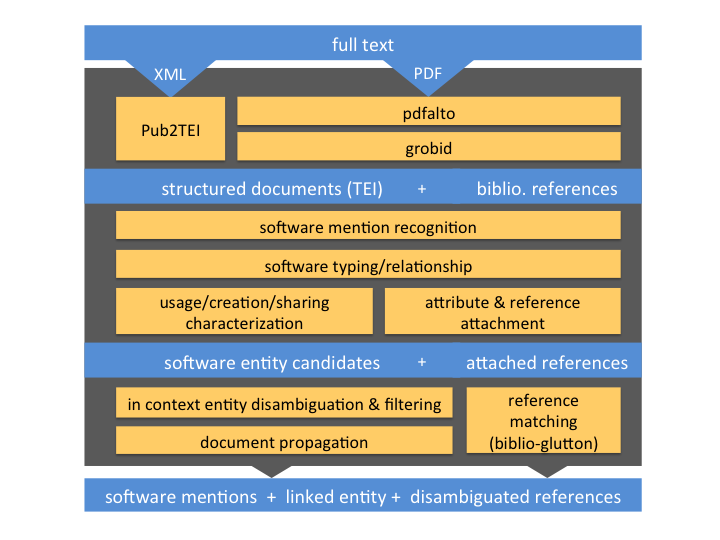
\includegraphics[width=0.7\textwidth,height=\textheight]{workflow_software_mention.png}
\caption{Overview of the Softcite software mention recognition process.}
\end{figure}

We expect input full texts to be in PDF formats, but a large range of
publisher XML formats are also supported. PDF are first parsed by a PDF
parser based on the Open source library Xpdf called \textbf{pdfalto}.
Complementary to the support of ALTO output, a modern format for OCR
output, pdfalto implements additional features relevant to scientific
documents, in particular better handling of multi-column documents, the
recognition of superscript/subscript style and the robust recognition of
line numbers for review manuscripts.

GROBID is then applied to structure the raw PDF stream into header,
sections, paragraphs, footnotes, etc. Grobid applies in cascade a set of
machine learning models to create hierarchical structures, combining
text content and layout features (e.g.~font and style information,
relative positions, SVG objects, etc.). Header metadata and all
bibliographical references are also extracted and parsed. If the input
is encoded in a publisher XML format, we transform the XML into the same
TEI format as produced by GROBID thanks to the Pub2TEI tool, which
support the main XML publisher formats such as JATS, Elsevier, Wiley,
etc. We can therefore centralize our document processing across PDF and
XML sources.

Mining for specific entities is only relevant to certain textual
structures of a scientific document, such as paragraphs, abstracts,
figure captions, etc. In the Softcite corpus, we calculated that, on
average, 28\% of publication content should be filtered out. This
includes metadata (author, affiliations), bibliographical sections,
table and figure content, formulas, headnotes, page numbers, reference
markers, or some editorial annexes (like conflicts of interest). Relying
on GROBID not only improve the quality of textual content, but it also
makes possible to apply the text mining process only to relevant
structures, avoiding a possible source of false recognition.

For relevant textual structures, a first NER mentions recognition is
applied to identify software names and related attributes. A second
model is then applied to refine the software mention types. Attachment
of the bibliographical references in the context of the software
mentions are evaluated and if successful these bibliographical
references are fully resolved against CrossRef DOI via the
\texttt{biblio-glutton} service. An entity disambiguation is realized in
context using \texttt{entity-fishing} for every software mention
candidates. If the candidates is significantly more likely scientific
entities different from a software, the candidates are discarded to
avoid likely false positives. Otherwise, if the software entity is a
known disambiguated software present in Wikidata, the entity is linked
via the resulting Q Wikidata identifier. Finally a document-level
propagation is realized to identified possible overlooked software name
matches in the same article in order to improve recall.

The additional external services used in the process:

\begin{itemize}
\item
  \textbf{biblio-glutton}, a large scale and fast bibliographical
  reference provision and matching service. Bibliographical references
  attached to software mentions are matched against CrossRef DOI using a
  2 stage approach: blocking based on fuzzy text matching and pairwise
  matching for bibliographical structure comparison.
\item
  \textbf{entity-fishing}, a Wikidata entity linking tool, used to
  disambiguate candidate software names in context. If the candidate
  name is disambiguated as an entity that is not a software with high
  confidence (e.g.~very likely the name of a protein or a project), we
  consider the candidate as a false positive and we filter it out. As a
  by-product, some positive candidates are disambiguated against known
  software present in Wikidata (around 12K software entities, excluding
  games), further enriching the extracted software mentions.
\end{itemize}

\hypertarget{evaluation}{%
\subsubsection{Evaluation}\label{evaluation}}

The following tables present the evaluation of the two main models
involved in the identification of software mentions, based on version
\texttt{0.7.2} of the Softcite software mention recognizer and the
updated version 2.0 of the Softcite dataset.

\textbf{Software mentions and attributes}

Similarly to the work in {[}17{]}, to evaluate the model on the actual
distribution of software mentions in scientific articles, we have reused
an \textbf{holdout set} containing the complete full text of 20\% the
Softcite Dataset documents (994 articles), reproducing the overall
distribution of documents with annotation (29.0\%), the distribution
between Biomedicine and Economics fields, and using a stratified
sampling to reproduce the overall distribution of mentions per document.
The \textbf{holdout set} reproduce therefore a realistic distribution of
software mentions and can be used to produce stable evaluation using
different version of the training data. We used the remaining 80\% of
documents (3,977 articles), divided at paragraph-level into positive
(1,886 paragraphs with at least one manual annotation) and negative
(612,597 paragraphs without manual annotations). To optimize the balance
between positive and negative sampling for the real distribution, the
final model was trained on the 1,886 positive paragraphs of the Softcite
dataset and a set a of 50,000 negative paragraphs selected with active
sampling as described in {[}17{]}.

Our best model is a fine-tuned LinkBERT base model {[}33{]} with an
additional CRF activation layer, which performs slighly but consistently
better for this task than a fine-tuned SciBERT model.

\begin{longtable}[]{@{}lllll@{}}
\toprule
& precision & recall & \textbf{F1-score} & support\tabularnewline
\midrule
\endhead
\textbf{publisher} & 75.51 & 88.80 & \textbf{81.62} & 250\tabularnewline
\textbf{software} & 74.01 & 88.98 & \textbf{80.81} & 989\tabularnewline
\textbf{url} & 53.97 & 82.93 & \textbf{65.38} & 41\tabularnewline
\textbf{version} & 83.99 & 90.81 & \textbf{87.27} & 283\tabularnewline
& & & &\tabularnewline
\textbf{all} (micro avg.) & 75.22 & 89.12 & \textbf{81.58} &
1563\tabularnewline
\bottomrule
\end{longtable}

\textbf{Software type refinement}

We report the evaluation of our best model for the typing of software
mentions, a fine-tuned SciBERT model with an additional CRF activation
layer. Because this model is applied only to sequences where at least
one software mention has been identified previously, the label
distribution of the input for prediction is the same as the one in the
training data. Scores are thus produced using 10-fold cross-validation
on a training set based on all the paragraph with at least one
annnotated software.

\begin{longtable}[]{@{}lllll@{}}
\toprule
& precision & recall & \textbf{F1-score} & support\tabularnewline
\midrule
\endhead
\textbf{component} & 71.43 & 71.43 & \textbf{71.43} & 7\tabularnewline
\textbf{environment} & 83.33 & 83.33 & \textbf{83.33} &
102\tabularnewline
\textbf{implicit} & 72.73 & 57.14 & \textbf{64.00} & 14\tabularnewline
\textbf{language} & 100.00 & 61.54 & \textbf{76.19} & 13\tabularnewline
& & & &\tabularnewline
\textbf{all} (micro avg.) & 82.81 & 77.94 & \textbf{80.30} &
136\tabularnewline
\bottomrule
\end{longtable}

\hypertarget{research-datasets}{%
\subsection{2.3 Research datasets}\label{research-datasets}}

\hypertarget{existing-work}{%
\subsubsection{Existing work}\label{existing-work}}

Following the success of CrossRef DOI for identifying publications, some
researchers have advocated for the use of persistent identifiers to
research datasets as a long-term solution to addressing data mention
detection and disambiguation {[}4{]}. However, in view of the slow
adoption and usage of PID for data citations, recent works are exploring
methods for detecting and linking informal data mentions from article
full-texts. Similarly to softare mentions, as data citations are
inconsistent, vague, incomplete and indirect {[}22{]}, detecting
information data citations must rely on NLP techniques, and more
particularly on the accurate and robust modern machine learning
techniques.

\ldots{} using GROBID {[}13{]}\ldots{} (however here dataset and model
not shared)

\textbf{NOTE: to be completed !}

\hypertarget{data-model-and-training-data-1}{%
\subsubsection{Data model and training
data}\label{data-model-and-training-data-1}}

Dataset mentions are usually less complex that software mentions, but
the exact scope of ``research datasets'' still varies from one existing
work/annotated corpus to another and needs some clarifications.

\hypertarget{implicit-versus-explicit-research-datasets}{%
\paragraph{Implicit versus explicit research
datasets}\label{implicit-versus-explicit-research-datasets}}

Although the production of various data is very common is a scientific
work, a large amount of the raw data discussed in scientific articles
are actually not named, not curated and not shared. For examples:

\begin{verbatim}
The 47 tilapia DNA samples were sent to Beijing Genome Institute (BGI) for 101 bp 
paired-end sequencing using Illumina Hiseq 2500. 
\end{verbatim}

The Illumina Hiseq 2500 device produces sequencing data, which are part
of the described study. These sequencing data are however not named and
not shared, they remain implicit.

We define this sort of research dataset as \emph{implicit dataset}.
These data are generally not considered as valuable by the researchers
and often not in a sharable state (proprietary format, embedded as
project resources). We consider fully automatic recognition of this kind
of datasets currently beyond what is feasable given the current existing
annotated corpus and machine learning technique accuracy.

In contrast, in this work, we focus on \emph{explicitly mentioned
datasets}: - named datasets - datasets without name, but explicitely
mentioned as existing data

\emph{Explicitly mentioned datasets} are research data identified as
such by the authors, discussed and considered valuable with respect to
the scientific claims of the publication and usually available in a form
that makes sharing possible.

\textbf{Ajouter un exemple}

\hypertarget{databases}{%
\paragraph{Databases}\label{databases}}

Is a mention to a database the same as a mention to a dataset? We
consider that the answer depends on the context, whether the research
work is actually refering to the data/dataset stored in the database or
more generally to the software or the service associated to the
database.

If some research data has been loaded and shared via this database, we
can can consider in general that this data are packaged as a dataset.

On the other hand, a ``dataset'' can exists independently from a
database management system and is not ambiguous with respect to its
storage and software access environment.

\hypertarget{data-sharing-initiativeproject}{%
\paragraph{Data sharing
initiative/project}\label{data-sharing-initiativeproject}}

It is frequent that a reference is made not and to a single dataset
(with a dataset name), but to a collection of datasets developed by this
initiative/project, with the name of a data sharing initiative/project.
For example the Coleridge Kaggle dataset (which is a particularly
imprecise and incomplete annotated corpus) is annotating the Alzheimer's
Disease Neuroimaging Initiative (ADNI) as a dataset name in the
following context:

\begin{verbatim}
Genome-wide pathway analysis of memory impairment in the Alzheimer’s Disease 
Neuroimaging Initiative (ADNI) cohort implicates gene candidates, canonical pathways, 
and networks.
\end{verbatim}

We consider however that this not a standard dataset citation. It
informs about the origin and location of some data used in the research
work, but does not describe precisely which data is considered.
Similarly, we can see references to a large
project/collaboration/experiments (collaboration in the sense of HEP or
Astronomy, such as ATLAS, CMS, LHCb), for actually referencing in
general data produced/shared by the collaboration and not the
collaboration itself. Such general reference is again not considered as
a dataset mention.

To summarize, we currently exclude these general mentions to such data
initiatives and projects from our dataset extraction. Only mentions to
individual research dataset or collection are considered as ``dataset''.

\hypertarget{accession-number}{%
\paragraph{Accession number}\label{accession-number}}

The references to an entry in a database, for instance via a unique
identifier such as an accession number is considered as a valid mention
to a dataset. The dataset here is defined by the combination of the data
service and the identifier. For example:

\begin{verbatim}
The RNA-seq data generated in this study have been deposited in DDBJ under accession 
codes DRA001101 and DRA004790."
\end{verbatim}

For a more detailed discussion and more examples, see
https://github.com/Barometre-de-la-Science-Ouverte/bso3-techdoc/blob/master/doc/scope\_and\_sharing.md

\hypertarget{annotations-1}{%
\paragraph{Annotations}\label{annotations-1}}

Developing an annotated corpus of dataset mentions entirely from scratch
would not have been possible for this project, given that the Softcite
dataset took several years of development and involved a total of 38
different human annotators. To train our dataset mention recognizer, we
reused existing annotated corpus, re-annotated them to follow our
guidelines and produce some additional annotations for a limited subset.

To tackle the sparsity problem, we could not take advantage of the full
text versions of the annotated articles. The existing training data are
sets of positive sentences with at least one dataset annotation. There
is no guarantee that the rest of these articles do not include other
datasets and checking such a large amount of content is highly
time-consuming. To mitiguate this issue, we separated the task in two
steps, the first one to identify the data sentences in a complete
article, and the second one to spot dataset mentions in selected data
sentences. This two steps approach was already implemented in the
DataSeer project and gave satisfactory performance. However, as the
DataSeer annotated data has not been released publicly, we reused and
developed ourself additional annotated data.

For the dataset mention recognition, we use the following resources:

\begin{itemize}
\item
  a re-annotated version of
  https://github.com/xjaeh/ner\_dataset\_recognition
  (\texttt{ner\_dataset\_recognition/}), a set of 6,000 sentences in the
  IR/ML/NLP domain with 3,684 dataset mentions. We fully reviewed the
  dataset and re-annotated to follow our dataset annotation principles:
  it covers now new datasets (not just reused ones) and annotation is at
  dataset level (avoid one annotation for a conjunction expression of
  datasets).
\item
  a set of approx. 1000 sentences from PubMed Central full-texts with at
  least one dataset mention (explicit and implicit datasets) and partial
  data acquisition device annotations.
\end{itemize}

These resources were used to train a LinkBERT base model {[}33{]} with
an additional CRF activation layer.

For the data sentence classification model, we used 2,000 positive
sentences containing at least one dataset mention and 20,000 negative
data sentences without dataset mention from PubMed Central full-texts
and from the Coleridge dataset.\footnote{https://www.kaggle.com/competitions/coleridgeinitiative-show-us-the-data/data}
This dataset was used to train a LinkBERT base model binary classifier.

\hypertarget{architecture-1}{%
\subsubsection{Architecture}\label{architecture-1}}

\begin{figure}
\centering
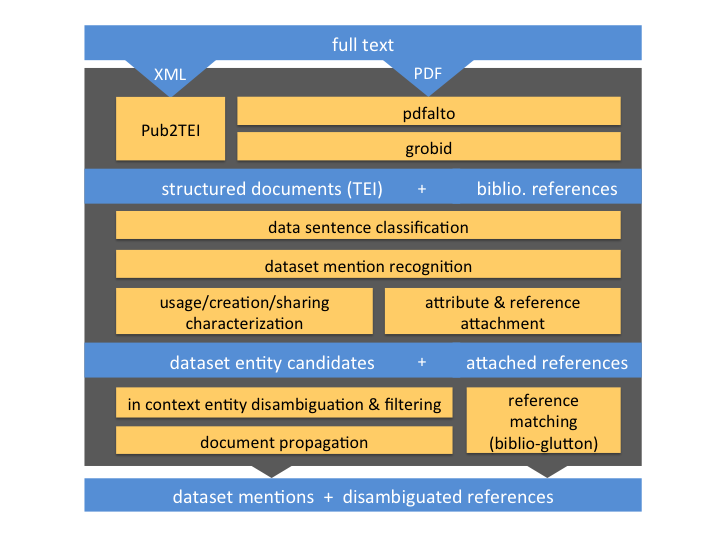
\includegraphics[width=0.7\textwidth,height=\textheight]{workflow_dataset_mention.png}
\caption{Overview of the DataStet dataset mention recognition process.}
\end{figure}

The architecture and process are very similar to the ones of software
mention recognition. The main difference is related to the two models
applied to recognize dataset mentions. A first classification model is
applied to every sentences of relevant section to determine if the
sentence is describing or not a dataset. The second model is applied on
positive data sentences to identify dataset mention spans and attributes
like URL and bibliographical references. This division of the
recognition task into two steps is introduced to mitigate the problem of
lack of annotations for complete documents, mentioned in the previous
section.

\hypertarget{current-performance}{%
\subsubsection{Current performance}\label{current-performance}}

As presented above, in order to manage sparcity of dataset mentions, a
first model is classifying if a sentence introduces a dataset or not. A
10-fold cross-validation on our dataset gives the following accuracy:

\begin{longtable}[]{@{}lllll@{}}
\toprule
& precision & recall & \textbf{F1-score} & support (10\%)\tabularnewline
\midrule
\endhead
\textbf{data setence} & 93.70 & 96.21 & 94.94 & 200\tabularnewline
\textbf{not data sentence} & 97.56 & 95.92 & 96.73 & 2000\tabularnewline
\bottomrule
\end{longtable}

Similarly, we evaluate the mention recognition using 10-fold
cross-validation on the annotated dataset. In the real application of
the models, the second model is applied only to sentences detected as
``data sentence'', so the error of the previous model detecting ``data
sentences'' will be propagated to the second model. However, even
combining the two error rates, the recognition of mentions of explicit
datasets (dataset with names or without name but expressed as dataset or
data) appears reliable with the current amount of training data. This
result confirms that indicators derived from these extracted mentions
can be build in a safe manner.

At this stage, implicit datasets are harder to recognize and will
require additional training data and modeling efforts. We also present
for reference the current recognition scores for data device mentions,
but their manual annotations are still work-in-progress and very
limited. We think that the automatic identification of data acquisition
devices or data processing devices could help in the future to spot
implicit data in a more reliable way.

\begin{longtable}[]{@{}lllll@{}}
\toprule
& precision & recall & \textbf{F1-score} & support (10\%)\tabularnewline
\midrule
\endhead
\textbf{explicit dataset} & 89.04 & 89.46 & \textbf{89.24} &
466\tabularnewline
\textbf{implicit dataset} & 71.85 & 67.15 & \textbf{69.38} &
927\tabularnewline
data device & 51.91 & 37.94 & 42.61 & 97\tabularnewline
\bottomrule
\end{longtable}

\hypertarget{characterization-of-mention-contexts}{%
\subsection{2.4 Characterization of mention
contexts}\label{characterization-of-mention-contexts}}

Whether or not a research dataset or software mentioned in an article
was used, created and shared is important to monitor the compliance with
Open Science policies. We hypothesize here that the wording used to
introduce and describe a dataset or software mention can characterize
its possible usage, creation and sharing. The sentences containing the
mentions are used as classifier input, without additional features. As
we observed that the wording used to describe the role of these mentions
is very similar for dataset and software, we use the same classifiers
for characterizing both research dataset and software mentions.

\hypertarget{training-data}{%
\subsubsection{Training data}\label{training-data}}

The annotated data for training the classifiers are a combination of
existing training data and additional manual annotation realized during
the project:

\begin{itemize}
\item
  l'attribut \emph{used} of the Softcite dataset
\item
  the corresponding annotations in the SoMeSci dataset
\item
  an additional set of 500 contexts manually annotated focusing more on
  datasets and the minoroty classes (\emph{created} and \emph{shared})
\end{itemize}

Table {[}{]} presents the distribution of classes in this training
dataset.

\begin{longtable}[]{@{}ll@{}}
\toprule
total contexts & 3,643\tabularnewline
\midrule
\endhead
used & 2,774\tabularnewline
not used & 869\tabularnewline
--- & ---\tabularnewline
created & 338\tabularnewline
not created & 3,305\tabularnewline
--- & ---\tabularnewline
shared & 266\tabularnewline
not shared & 3,377\tabularnewline
\bottomrule
\end{longtable}

\hypertarget{current-performance-1}{%
\subsubsection{Current performance}\label{current-performance-1}}

The following scores are thus produced using 10-fold cross-validation
based on three binary classifiers, one per class used/created/shared.
The classifiers are fine-tuned LinkBERT base model {[}33{]}. Binary
classifiers for each class perform significantly better than a single
multiclass classifier (up to 4 F1-score points).

\begin{longtable}[]{@{}lllll@{}}
\toprule
& precision & recall & \textbf{F1-score} & support\tabularnewline
\midrule
\endhead
\textbf{used} & 96.83 & 94.18 & \textbf{95.49} & 292\tabularnewline
\textbf{not used} & 84.40 & 91.09 & \textbf{87.62} & 101\tabularnewline
--- & --- & --- & --- & ---\tabularnewline
\textbf{created} & 81.08 & 83.33 & \textbf{82.19} & 31\tabularnewline
\textbf{not created} & 98.31 & 98.04 & \textbf{98.18} &
362\tabularnewline
--- & --- & --- & --- & ---\tabularnewline
\textbf{shared} & 81.82 & 90.00 & \textbf{85.71} & 26\tabularnewline
\textbf{not shared} & 99.35 & 98.71 & \textbf{99.03} &
385\tabularnewline
\bottomrule
\end{longtable}

\hypertarget{recognition-of-availability-statements}{%
\subsection{2.5 Recognition of availability
statements}\label{recognition-of-availability-statements}}

We have extended GROBID to identify automatically data and code
availability statements in research publications. We define a data
and/or code availability statements as a standalone section of a
research publication (with a section title and one or several
paragraphs) describing how the data and code involved in the research
work can or cannot be accessed. We consider no restriction on the types
of data described in the sharing statement, e.g.~a section describing
the accession numbers from a scientific database corresponding to
research data used in a research work will be considered as a data
availability statement.

Availability statements appear usually in the front page of an article
or at the end as a annex, but we also considered positions inside the
main body, which are actually not rare in preprints. We do not put any
constraints on the section title associated to ``data availability
statements''. It appears that, especially in preprints, this section can
be introduce with a vast variety of section titles.

95 articles out of the 520 training articles of the GROBID
\texttt{segmentation} model have been further annotated with data
availability section markups. This GROBID model is used to segment the
main zone of a scientific article, such as header, body, bibliographical
section, acknowledgement or funding. The data availability section is
then structured and identified as such in the file TEI result file.

We evaluated the reliability of recognition on two sets, one
corresponding to high quality publisher publications, and one with only
preprints at the other end of the spectrum of difficulty:

\begin{itemize}
\item
  a set of 1000 random PLOS articles in PDF and JATS XML (from the
  complete PLOS collection) containing 779 data and code availability
  statement markup information
\item
  a set of 984 random eLife articles in PDF and JATS XML (from the
  complete eLife collection) containing 585 data availability statements
  markup information
\item
  a set of 2000 bioRxiv articles, which have been reviewed and completed
  manually regarding data and code availability statement markup,
  containing 473 data availability statements
\end{itemize}

Note that the markup information and encoding available in the publisher
or bioRxiv XML is not always 100\% accurate, because the content of the
XML and the PDF versions can slightly change, and the XML can typically
contain more information than what is in the PDF (for instance eLife XML
contain the author keywords, while they are not present in the final
published PDF). However, although we do not obtain perfect absolute
evaluation scores, comparing automatic extraction from PDF with the
publisher XML give a good estimation of the extraction accuracy in
general.

The bioRxiv set can be seen as the most challenging in general because,
as a set of preprints, the authors are at this stage more or less free
to format and express data availability statements as they want. In
contrast, for published articles such as PLOS or eLife, the section
title of data and code availability statements is constrained by the
publisher format and thus much easier to recognize.

Table {[}{]} presents an evaluation of the accuracy of the data and code
availability statement recognition in a end-to-end scenario (starting
with PDF as input).

\begin{longtable}[]{@{}lllll@{}}
\toprule
collection & precision & recall & \textbf{F1-score} &
support\tabularnewline
\midrule
\endhead
\textbf{PLOS 1000 articles} & 99.57 & 89.73 & \textbf{94.4} &
779\tabularnewline
\textbf{eLife 984 articles} & 96.62 & 92.82 & \textbf{94.68} &
585\tabularnewline
\textbf{bioRxiv 2000 articles} & 82.7 & 78.25 & \textbf{80.41} &
473\tabularnewline
\bottomrule
\end{longtable}

We observed that on recent publications (2020 and after), the presence
of data availability sections is correctly recognized in nearly all PLOS
and eLife. On the other hand, preprint data availability statements can
be challenging to identify because they can appear in non-usual position
in the article (e.g.~inside the article body) and can be introduced by a
large variety of section titles depending on the described data. In
published versions, we generally observe a high regularity and very high
precision similar to PLOS/eLife articles.

\hypertarget{matching-and-aggregation}{%
\subsection{2.6 Matching and
aggregation}\label{matching-and-aggregation}}

At document-level.

At corpus-level, disambiguating mentions of the same dataset or software
in different documents could lead to indicators at the level of produced
dataset and software. Such overall index of research dataset and
software is currently out of the scope of the selected indicators.

\hypertarget{monitoring-indicators-construction}{%
\subsection{2.7 Monitoring indicators
construction}\label{monitoring-indicators-construction}}

To help steer French public policy, the BSO must have indicators that
meet several conditions:

\begin{itemize}
\item
  indicators that evolve ``quickly'' according to changes in uses and
  practices (indicators with little temporal inertia)
\item
  indicators that are easily understandable and interpretable
\item
  indicators whose floor and ceiling are known in advance and which are
  achievable.
\end{itemize}

For example, for the publications component, the BSO looks at the
percentage of open access publications for the previous year: each year
the new indicator does not depend on previous years. It varies between
0\% and 100\%, and 100\% is the target for 2030.

Although the subject is more complex, it is important that the same
applies to indicators for research data and software. The detection work
uses the full-text PDFs of the publications as raw material. It is
therefore natural to propose indicators relating to the proportion of
publications. As the methodology is similar for both datasets and
software, the proposed indicators will be equivalent, replacing each
time dataset by software. A ``naive'' indicator would be, for example,
the proportion of publications that share a dataset :

\[ I_{naive} = {\text{number of publications that 'shares' a dataset} \over \text{total number of publications}} \]

This indicator is simple, but has several shortcomings:

\begin{itemize}
\item
  first, concerning the denominator, not all publications can be
  analysed by Softcite / DataStet, because the PDF could not
  systematically be downloaded (closed access for which we do not have a
  subscription, missing PDF, etc \ldots). It should therefore be
  replaced at least by the number of publications that have been
  analysed.
\item
  secondly, we want to have an indicator whose upper bound has a meaning
  linked to the objectives of the public policy. For example, an article
  for which the research work did not require the use of any dataset
  cannot share it.
\end{itemize}

Thus, the notion of a publication that shares a dataset should be
clarified as a publication that uses, creates and shares a dataset.

We therefore propose to monitor a modified key indicator:

\[ I_{share} = {\text{number of publications that use, create and share a dataset} \over \text{number of publications analyzed that use and create a dataset}} \]

The disadvantage of reasoning in this way is that we lose some of the
lessons that could be learned from the non-actionable part of the scope
(publications that do not create a dataset). This is why we propose to
complete the analysis with two additional indicators:

\[ I_{create} = {\text{number of publications that use and create a dataset} \over \text{number of publications analyzed that use a dataset}} \]

and

\[ I_{use} = {\text{number of publications that use a dataset} \over \text{number of publications analyzed}} \]

These three indicators therefore make it possible to have a global and
decomposable view of all the cases: the top of the pyramid, which is
actionable, and which we want to increase. The other two are more
descriptive, but will provide a better understanding of practices and
uses, particularly by breaking them down by subject area.

We note in particular that we find the naive indicator initially
proposed as follows:

\[ I_{naive} = I_{share} \times I_{create} \times I_{use} \times P_{analyzed} \]

where

\[ P_{analyzed} = {\text{number of publications analyzed} \over \text{total number of publications}} \]

All these indicators can be broken down by the components linked to the
publications themselves: year of publication, disciplines, publishers
etc. Monitoring by year of publication (rather than the full stock of
publications since the 2010s) allows for a responsive indicator.

We supplement these indicators with a simpler one, linked simply to the
presence, in the structure of the full text, of an explicit Data
Availibility Statement paragraph (which in no way guarantees sharing)
but nevertheless makes it possible to observe the evolution of this
practice (which is very much linked to the publication's editor).

\newpage

\hypertarget{implementation}{%
\section{3. Implementation}\label{implementation}}

Architecture diagram

\begin{figure}
\centering
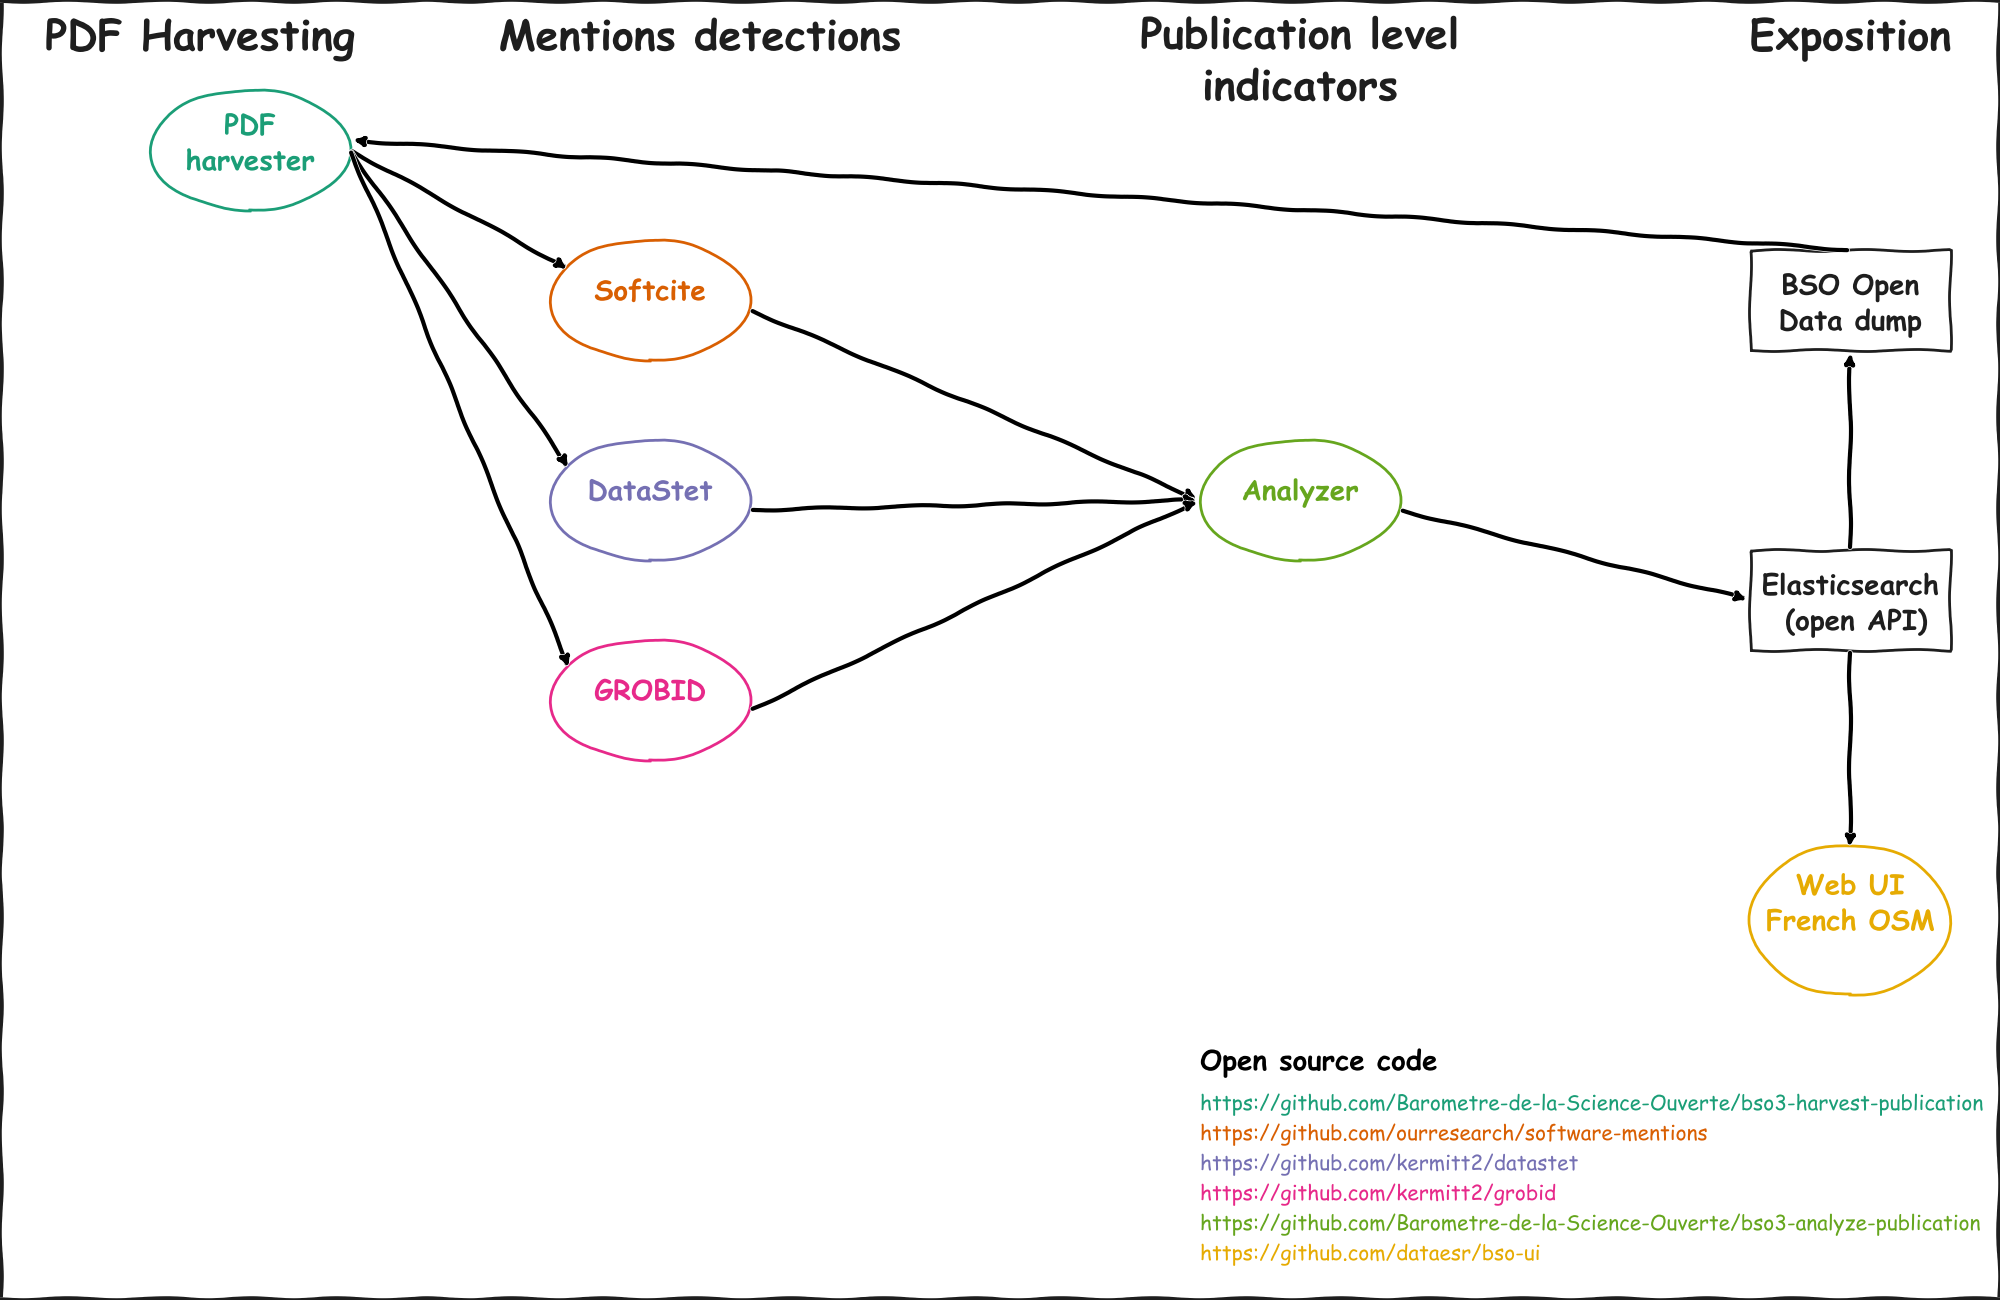
\includegraphics[width=6.25in,height=\textheight]{https://raw.githubusercontent.com/Barometre-de-la-Science-Ouverte/bso3-techdoc/master/methodology/flow_chart_publications_bso3.png}
\caption{Global overview of the publications data flows}
\end{figure}

Workflow description

Infrastructure and runtime indications

\hypertarget{results}{%
\section{4. Results}\label{results}}

\hypertarget{full-text-harvesting}{%
\subsection{4.1 Full text harvesting}\label{full-text-harvesting}}

\begin{longtable}[]{@{}lcrr@{}}
\toprule
is\_oa & number of publications & number of PDF downloaded & \% download
success\tabularnewline
\midrule
\endhead
True & 698,610 & 616,733 & 88 \%\tabularnewline
False & 659,584 & 272,070 & 41 \%\tabularnewline
Total & 1,358,194 & 888,803 & 65 \%\tabularnewline
\bottomrule
\end{longtable}

\begin{longtable}[]{@{}lcr@{}}
\toprule
harvester\_type & number of PDF downloaded & \% of total\tabularnewline
\midrule
\endhead
standard & 559,332 & 63 \%\tabularnewline
Elsevier TDM API & 200,155 & 22 \%\tabularnewline
arXiv & 78,078 & 9 \%\tabularnewline
Wiley TDM API & 51,238 & 6 \%\tabularnewline
\bottomrule
\end{longtable}

\hypertarget{dataset-and-software-mention-extraction}{%
\subsection{4.2 Dataset and software mention
extraction}\label{dataset-and-software-mention-extraction}}

\hypertarget{research-product-deduplication}{%
\subsection{4.3 Research product
deduplication}\label{research-product-deduplication}}

\hypertarget{french-open-science-monitor-indicators-and-dashboards}{%
\subsection{4.4 French Open Science Monitor indicators and
dashboards}\label{french-open-science-monitor-indicators-and-dashboards}}

\ldots{}

One of the ojectives of the French Open Science Monitor is to provide
all research institutions with a local version of the indicators.
Similarly as for measuring the openness of research publications on the
existing platform, the new indicators can be bounded to datasets and
software produced by the researchers only affiliated to a particular
organization. The ability to measure the research activity at different
scale, from a given organization to the national level has led to the
creation of a BSO user group
(https://groupes.renater.fr/sympa/info/bso-etablissements).

\hypertarget{limitations-and-future-work}{%
\subsection{5 Limitations and future
work}\label{limitations-and-future-work}}

\hypertarget{limitations}{%
\subsubsection{5.1 Limitations}\label{limitations}}

\hypertarget{future-work}{%
\subsubsection{5.2 Future work}\label{future-work}}

\hypertarget{domain-coverage}{%
\paragraph{5.2.1 Domain coverage}\label{domain-coverage}}

Research datasets and software mention recognizers are limited by the
poor multidisciplinary coverage of the training data. {[}17{]} shows
that the recognition performance falls by around 20 points F1-score on a
new scientific domain.

\hypertarget{large-scale-research-entity-disambiguation}{%
\paragraph{5.2.2 Large-scale research entity
disambiguation}\label{large-scale-research-entity-disambiguation}}

\hypertarget{local-open-science-monitor}{%
\paragraph{5.2.3 Local Open Science
Monitor}\label{local-open-science-monitor}}

\hypertarget{data-and-software-availability}{%
\section{Data and software
availability}\label{data-and-software-availability}}

The data resulting from this work are publicly available on the French
Ministry of Higher Education and Research open data portal:

The source code used for the French Open Science Monitor is available on
GitHub, and shared with open source licences.

\hypertarget{acknowledgements}{%
\section{Acknowledgements}\label{acknowledgements}}

The extension of the French Open Science Monitor (BSO) presented in this
document was supported by France Relance/NextGenerationEU funding.

Previous work on the Softcite dataset and the Softcite Software mention
recognizer was supported by the Alfred P. Sloan Foundation, Grant/Award
Number: 2016-7209 (2018-2020) and the Gordon and Betty Moore Foundation,
Grant/Award Number 8622 (2021). We also acknowledge the Jetstream cloud
environment part of XSEDE and the Texas Advanced Computing Center (TACC)
at The University of Texas at Austin for providing computing resources
that have contributed to the creation of these resources in 2021.
DataStet is a fork of dataseer-ml, developed in the context of the
DataSeer project (2019-2020), supported by the Alfred P. Sloan
Foundation.

\hypertarget{references}{%
\section*{References}\label{references}}
\addcontentsline{toc}{section}{References}

\hypertarget{refs}{}
\begin{cslreferences}
\leavevmode\hypertarget{ref-beltagy2019scibert}{}%
{[}1{]} Beltagy, I. et al. 2019. SciBERT: A pretrained language model
for scientific text.

\leavevmode\hypertarget{ref-bracco_extending_2022}{}%
{[}2{]} Bracco, L. et al. 2022. Extending the open monitoring of open
science: A new framework for the French Open Science Monitor (BSO).
(2022).

\leavevmode\hypertarget{ref-10.5555ux2f1870658.1870756}{}%
{[}3{]} Chiticariu, L. et al. 2010. Domain adaptation of rule-based
annotators for named-entity recognition tasks. \emph{Proceedings of the
2010 conference on empirical methods in natural language processing}
(USA, 2010), 1002--1012.

\leavevmode\hypertarget{ref-10.5334ux2fdsj-2019-009}{}%
{[}4{]} Cousijn, F., H. and Simons, N. 2019. Bringing citations and
usage metrics together to make data count. \emph{Data Science Journal}.
18, 1 (2019), 9.
DOI:\url{https://doi.org/http://doi.org/10.5334/dsj-2019-009}.

\leavevmode\hypertarget{ref-10.7717ux2fpeerj-cs.835}{}%
{[}5{]} David, S. et al. The role of software in science: A knowledge
graph-based analysis of software mentions in PubMed Central. \emph{PeerJ
Computer Science}. 8, e835.
DOI:\url{https://doi.org/10.7717/peerj-cs.835}.

\leavevmode\hypertarget{ref-devlin2018bert}{}%
{[}6{]} Devlin, J. et al. 2018. BERT: Pre-training of deep bidirectional
transformers for language understanding.

\leavevmode\hypertarget{ref-du_softcite_2021}{}%
{[}7{]} Du, C. et al. 2021. Softcite dataset: A dataset of software
mentions in biomedical and economic research publications. \emph{Journal
of the Association for Information Science and Technology}. 72, 7 (Jul.
2021), 870--884. DOI:\url{https://doi.org/10.1002/asi.24454}.

\leavevmode\hypertarget{ref-du_peerj_2022}{}%
{[}8{]} Du, C. et al. Understanding progress in software citation: A
study of software citation in the CORD-19 corpus. \emph{PeerJ Computer
Science}. 8, e1022. DOI:\url{https://doi.org/10.7717/peerj-cs.1022}.

\leavevmode\hypertarget{ref-he_han_2017}{}%
{[}9{]} He, L. and Han, Z. 2017. Do usage counts of scientific data make
sense? An investigation of the dryad repository. \emph{Library Hi Tech}.
35, 2 (2017), 332--342.
DOI:\url{https://doi.org/10.1108/LHT-12-2016-0158}.

\leavevmode\hypertarget{ref-howison_software_2016}{}%
{[}10{]} Howison, J. and Bullard, J. 2016. Software in the Scientific
Literature: Problems with Seeing, Finding, and Using Software Mentioned
in the Biology Literature. \emph{Journal of the Association for
Information Science and Technology}. 67, 9 (2016), 2137--2155.
DOI:\url{https://doi.org/10.1002/asi.23538}.

\leavevmode\hypertarget{ref-istrate_2022}{}%
{[}11{]} Istrate, A.-M. et al. 2022. A large dataset of software
mentions in the biomedical literature. arXiv.

\leavevmode\hypertarget{ref-kruger_literature_2020}{}%
{[}12{]} Krüger, F. and Schindler, D. 2020. A Literature Review on
Methods for the Extraction of Usage Statements of Software and Data.
\emph{Computing in Science Engineering}. 22, 1 (Jan. 2020), 26--38.
DOI:\url{https://doi.org/10.1109/MCSE.2019.2943847}.

\leavevmode\hypertarget{ref-10.1002ux2fpra2.614}{}%
{[}13{]} Lafia, S. et al. 2022. A natural language processing pipeline
for detecting informal data references in academic literature.
\emph{Proceedings of the Association for Information Science and
Technology}. 59, 1 (2022), 169--178.
DOI:\url{https://doi.org/https://doi.org/10.1002/pra2.614}.

\leavevmode\hypertarget{ref-Larregue_2020}{}%
{[}14{]} Larregue, Julien, Vincent-Lamarre, Philippe, Lebaron, Frédéric
and Larivière, Vincent 2020. Covid-19: where is the data? Impact of
Social Sciences Blog.

\leavevmode\hypertarget{ref-LAURINAVICHYUTE2022104332}{}%
{[}15{]} Laurinavichyute, A. et al. 2022. Share the code, not just the
data: A case study of the reproducibility of articles published in the
journal of memory and language under the open data policy. \emph{Journal
of Memory and Language}. 125, (2022), 104332.
DOI:\url{https://doi.org/https://doi.org/10.1016/j.jml.2022.104332}.

\leavevmode\hypertarget{ref-LeeDeleris:2020}{}%
{[}16{]} Lee, J. and Deleris, L. 2020. Sequencing, combining and
sampling classifiers to help find needles in haystacks. \emph{24th
european conference on artificial intelligence, ecai} (Santiago de
Compostela, Spain, Sep. 2020).

\leavevmode\hypertarget{ref-10.1145ux2f3459637.3481936}{}%
{[}17{]} Lopez, P. et al. 2021. Mining software entities in scientific
literature: Document-level NER for an extremely imbalance and
large-scale task. \emph{Proceedings of the 30th acm international
conference on information \& knowledge management} (New York, NY, USA,
2021), 3986--3995.

\leavevmode\hypertarget{ref-macgregor2022exploring}{}%
{[}18{]} Macgregor, G. et al. 2022. Exploring the concept of pid
literacy: User perceptions and understanding of persistent identifiers
in support of open scholarly infrastructure. \emph{arXiv preprint
arXiv:2211.07367}. (2022).

\leavevmode\hypertarget{ref-McKenzie_2017}{}%
{[}19{]} McKenzie, L. 2017. Want to analyze millions of scientific
papers all at once? Here's the best way to do it. \emph{Science}. (Jul.
2017). DOI:\url{https://doi.org/10.1126/science.aan7139}.

\leavevmode\hypertarget{ref-mesri_2nd_2021}{}%
{[}20{]} MESR 2021. 2nd National Plan for Open Science.

\leavevmode\hypertarget{ref-mesri_national_2018}{}%
{[}21{]} MESR 2018. National Plan for Open Science.

\leavevmode\hypertarget{ref-10.1087ux2f20110204}{}%
{[}22{]} MOONEY, H. 2011. Citing data sources in the social sciences: Do
authors do it? \emph{Learned Publishing}. 24, 2 (2011), 99--108.
DOI:\url{https://doi.org/https://doi.org/10.1087/20110204}.

\leavevmode\hypertarget{ref-10.1002ux2fasi.24049}{}%
{[}23{]} Park, H. et al. 2018. Informal data citation for data sharing
and reuse is more common than formal data citation in biomedical fields.
\emph{Journal of the Association for Information Science and
Technology}. 69, 11 (2018), 1346--1354.
DOI:\url{https://doi.org/https://doi.org/10.1002/asi.24049}.

\leavevmode\hypertarget{ref-olivier_philippe_2019_2585783}{}%
{[}24{]} Philippe, O. et al. 2019. softwaresaved/international-survey:
Public release for 2018 results. Zenodo.

\leavevmode\hypertarget{ref-10.5334ux2fdsj-2020-042}{}%
{[}25{]} Riedel, N. et al. 2020. ODDPub - a text-mining algorithm to
detect data sharing in biomedical publications. \emph{Data Science
Journal}. 19, 1 (2020), 42.
DOI:\url{https://doi.org/http://doi.org/10.5334/dsj-2020-042}.

\leavevmode\hypertarget{ref-10.1145ux2f3459637.3482017}{}%
{[}26{]} Schindler, D. et al. 2021. SoMeSci- a 5 star open data gold
standard knowledge graph of software mentions in scientific articles.
\emph{Proceedings of the 30th acm international conference on
information \& knowledge management} (New York, NY, USA, 2021),
4574--4583.

\leavevmode\hypertarget{ref-science_2011}{}%
{[}27{]} Science staff 2011. Challenges and opportunities.
\emph{Science}. 331, 6018 (2011), 692--693.
DOI:\url{https://doi.org/10.1126/science.331.6018.692}.

\leavevmode\hypertarget{ref-10.1371ux2fjournal.pbio.3001107}{}%
{[}28{]} Serghiou S, Contopoulos-Ioannidis DG, Boyack KW, Riedel N,
Wallach JD, Ioannidis JPA 2021. Assessment of transparency indicators
across the biomedical literature: How open is open? \emph{PLoS Biol}.
19, 3 (2021), e3001107.
DOI:\url{https://doi.org/https://doi.org/10.1371/journal.pbio.3001107}.

\leavevmode\hypertarget{ref-10.1371ux2fjournal.pone.0134826}{}%
{[}29{]} Tenopir, E.D.A.A., Carol AND Dalton 2015. Changes in data
sharing and data reuse practices and perceptions among scientists
worldwide. \emph{PLOS ONE}. 10, 8 (Aug. 2015), 1--24.
DOI:\url{https://doi.org/10.1371/journal.pone.0134826}.

\leavevmode\hypertarget{ref-2020200105714T}{}%
{[}30{]} Trienes, J. et al. 2020. Comparing Rule-based, Feature-based
and Deep Neural Methods for De-identification of Dutch Medical Records.
\emph{Proceedings of the 1st acm wsdm health search and data mining
workshop (hsdm2020)} (2020).

\leavevmode\hypertarget{ref-VANDEWIELE2021101987}{}%
{[}31{]} Vandewiele, G. et al. 2021. Overly optimistic prediction
results on imbalanced data: A case study of flaws and benefits when
applying over-sampling. \emph{Artificial Intelligence in Medicine}. 111,
(2021), 101987.
DOI:\url{https://doi.org/https://doi.org/10.1016/j.artmed.2020.101987}.

\leavevmode\hypertarget{ref-Westergaard_2017}{}%
{[}32{]} Westergaard, D. et al. 2017. Text mining of 15 million
full-text scientific articles. (Jul. 2017).
DOI:\url{https://doi.org/10.1101/162099}.

\leavevmode\hypertarget{ref-yasunaga2022linkbert}{}%
{[}33{]} Yasunaga, M. et al. 2022. LinkBERT: Pretraining language models
with document links. \emph{Association for computational linguistics
(acl)} (2022).
\end{cslreferences}


\end{document}
